\documentclass[sigconf,anonymous,review]{acmart}
\usepackage{popets}

\setcopyright{popets}
\copyrightyear{2027}

\acmYear{2027}
\acmVolume{2027}
\acmNumber{X}
\acmDOI{XXXXXXX.XXXXXXX}
\acmISBN{}
\acmConference{Proceedings on Privacy Enhancing Technologies}
\settopmatter{printacmref=false,printccs=false,printfolios=true}

% --- Math and algorithm support (acmart already loads amsmath, amssymb, etc.) ---
\usepackage{amsthm}
\usepackage{mathtools}
\usepackage{algorithm}
\usepackage[noend]{algpseudocode}
\usepackage{enumitem}
\usepackage{tikz}
\usepackage{pgfplots}
\pgfplotsset{compat=1.18}
\usetikzlibrary{arrows.meta, positioning, fit, backgrounds, calc}

% --- Theorem environments ---
\newtheorem{theorem}{Theorem}
\newtheorem{lemma}[theorem]{Lemma}
\newtheorem{proposition}[theorem]{Proposition}
\newtheorem{corollary}[theorem]{Corollary}
\theoremstyle{definition}
\newtheorem{definition}[theorem]{Definition}
\newtheorem{assumption}[theorem]{Assumption}
\theoremstyle{remark}
\newtheorem{remark}[theorem]{Remark}

% --- Notation macros (from IEEEtran version) ---
\newcommand{\R}{\mathbb{R}}
\newcommand{\E}{\mathbb{E}}
\newcommand{\Prob}{\mathbb{P}}
\newcommand{\eps}{\varepsilon}
\newcommand{\model}{\theta}
\newcommand{\summary}{\sigma}
\newcommand{\clip}{\mathrm{clip}}
\newcommand{\indist}{\stackrel{(\eps,\delta)}{\approx}}
\newcommand{\clientset}{\mathcal{C}}
\newcommand{\forget}{i^{\star}}

\begin{document}

\title[FORGE: FCL with Formal Guarantees]{FORGE: A Protocol for Federated Continual Unlearning with Formal Guarantees}

\author{Anonymous Author(s)}
\affiliation{%
  \institution{Anonymised for review}
  \city{Anonymised}
  \country{Anonymised}}
\email{anonymised@example.com}

\renewcommand{\shortauthors}{Anonymous}

\begin{abstract}
When a client leaves a federated learning system, the right-to-erasure obligation
asks the server to remove that client's influence from the shared model. Existing
federated unlearning methods force a trade: they either store every past client
update (breaking secure aggregation), need the departing client to come back
online, or lack a formal privacy guarantee. FORGE makes forgetting a property of
the training dynamics. The shared feature extractor is updated by a decayed
aggregation that causes each client's residual contribution to fade on its
own; alongside it, each client pre-commits a tiny noisy summary of their data.
At erasure time, the server performs a single bounded step on the classifier
head using the departing client's summary. The two mechanisms compose under
Gaussian differential privacy to give an auditable guarantee a supervisory
authority can verify. On a 3-seed CIFAR-10 benchmark at realistic utility,
FORGE matches full retraining in both accuracy and membership-inference
resistance, and processes each erasure request in $0.28$ seconds --- around
fifty times faster than the fastest history-based baseline, and five orders of
magnitude faster than SIFU with proper replay. Cross-dataset runs on CIFAR-100
and FEMNIST reproduce the ordering.
\end{abstract}


\keywords{federated learning, machine unlearning, differential privacy, right to erasure, GDPR}

\maketitle

\section{Introduction}
\label{sec:introduction}

\paragraph{Real-world privacy relevance.}
This paper addresses the right-to-erasure obligation of GDPR Article~17 as applied to
federated models under EDPB Opinion 28/2024 on AI systems \cite{edpb2024}, which
requires data controllers to evidence that a departing client's residual influence on
any downstream model is negligible. In cross-institutional and cross-device federated
learning deployments (medical, financial, keyboard, smart-home), this obligation is
operationally difficult: the server cannot observe raw client data by design, and
retraining from scratch is prohibitive. The protocol proposed here, FORGE, provides
a formal $(\varepsilon, \delta)$-indistinguishability guarantee that a supervisory
authority can verify without the controller publishing a pre-erasure model, and
without requiring the departing client to remain online. The guarantee, the
verification protocol (Section~\ref{sec:method-erasure}), and the cross-release
composition analysis (Section~\ref{sec:theory}) are the components that make the
protocol deployable as a compliance mechanism for live FL systems rather than as a
theoretical construction.

The right to erasure obliges a data controller to remove personal data on request and,
under recent guidance, to evidence that residual influence on any downstream model is
negligible \cite{edpb2024}. In Federated Learning (FL), and especially in Federated
Continual Learning (FCL), operationalising this obligation is complicated by the very
properties that make FL privacy-preserving in the first place. Secure aggregation
prevents the server from observing individual client updates \cite{bonawitz2017};
asynchronous or streaming continual learning spreads a client's influence across weights,
aggregated statistics, replay buffers, and distilled knowledge \cite{yoon2021}; and
empirical work has shown that secure aggregation is not, on its own, sufficient
protection against membership inference \cite{pillutla2023}. Any credible Federated
Unlearning (FU) procedure must therefore not merely alter the model, but do so in a way
that a supervisory authority, as well as the departing client themselves, can verify
without introducing new avenues of leakage.

Existing FU methods trade among three costs, and no prior work eliminates all three
simultaneously. First, \emph{history-based} methods reconstruct or calibrate a model
without the departing client using stored per-round updates or gradients
\cite{liu2021federaser,fraboni2024sifu,zhang2023fedrecovery}. This gives the tightest
fidelity to a retrained model, but the storage itself is at odds with secure aggregation
and, under EDPB Opinion 28/2024, may not qualify as anonymous processing. In
cross-device deployments with millions of clients, it is also often infeasible. Second,
\emph{interactive} methods avoid storage by having the departing client re-engage with
the server: gradient ascent on their local data with a distance constraint from the
global model \cite{halimi2022}. This is elegant but assumes the client's continued
participation, which is an assumption that fails precisely when the client is exercising
a right to leave. Third, \emph{heuristic} methods (weight negation, pruning,
random-label perturbation) sidestep both storage and cooperation but offer no formal
guarantee a controller can evidence \cite{khalil2025not,gu2024fedau}. Recent
memorisation-scoped approaches \cite{wei2026fedmemprune} give strong empirical fidelity
but do not currently ship with a provable indistinguishability bound.

A separate, less-recognised failure mode is that the unlearning procedure itself leaks.
Publishing (or letting a client observe) a before/after model pair enables membership
inference attacks (MIA) that outperform attacks on the original model
\cite{chen2021unlearningleaks}, and dedicated federated attacks such as the Federated
Unlearning Inversion Attack (FUIA) exploit exactly this signal \cite{fuia2025}. Any
method that requires a comparable ``after'' model to be released must be evaluated
against this channel.

In this paper, we propose FORGE (\textbf{For}ward-forgetting via decayed aggregation and
pre-committed erasure summaries), an FCL protocol under which the erasure guarantee is a
property of the training dynamics, rather than a procedure invoked at request time. The
protocol has two ingredients. (1)~\emph{Bounded-influence decay.} We formalise a
training-time property called $(\varepsilon, \delta, T)$-forward forgetting: a client
that departs at round $r$ is $(\varepsilon, \delta)$-indistinguishable from a
counterfactual training run that never included them, by round $r + T$. Under a decayed
aggregation protocol with per-round clipping constant $C$ and calibrated server noise
$\sigma$, we exhibit an explicit rate $\varepsilon_1(T)$. This is the FL-native analogue
of the DP-as-unlearning line \cite{guo2020certified,sekhari2021remember,neel2021descent},
but time-indexed rather than budgeted once-for-all. (2)~\emph{Pre-committed differentially
private (DP) summary channel.} During training, each client submits alongside their
gradient a small DP summary $\sigma_i$ of their local data distribution. At erasure time,
the server uses $\sigma_{\forget}$ to perform a non-interactive subtraction of the
client's memorised residual, at additional cost $\varepsilon_2$. No per-round updates
are stored, and no interaction with the client is required at or after the request.
Because the feature-block aggregation and the summary channel use independent Gaussian
noise sources, and because the summary-subtraction step at erasure time operates only
on the head, adaptive Gaussian-DP composition applies and gives a
$\sqrt{\mu_1(T)^2 + \mu_\summary^2}$-GDP joint release as the overall formal guarantee.

\paragraph{Contributions.}
\begin{enumerate}[leftmargin=*,itemsep=2pt]
\item A new privacy definition: $(\varepsilon, \delta, T)$-forward forgetting, the first
per-client, time-indexed unlearning guarantee for federated (continual) learning
(Def.~\ref{def:forward-forgetting}).
\item A decayed aggregation FCL protocol with per-round clipping and calibrated server
noise that achieves forward forgetting at an explicit rate
(Alg.~\ref{alg:decayed-aggregation}).
\item A pre-committed DP summary construction that enables non-interactive server-side
subtraction of a departed client's memorised residual, with no per-round update storage
and no request-time client cooperation (Alg.~\ref{alg:erasure}).
\item A composition theorem (Thm.~\ref{thm:composition}) that yields a
$\sqrt{\mu_1(T)^2 + \mu_\summary^2}$-GDP guarantee by adaptive Gaussian-DP
composition, enabled by the independent Gaussian noise sources of the feature-block
and summary mechanisms in Algorithm~\ref{alg:decayed-aggregation}.
\item An empirical evaluation whose primary benchmark is CIFAR-10 non-IID
stationary FL (ResNet-18, 100 clients, 200 rounds, Dirichlet $\alpha{=}0.3$, three
seeds) at realistic deployment utility, with a class-incremental stress test
comparing FORGE against eleven baselines including an $\varepsilon$-sweep of
FedRecovery across $\varepsilon \in \{1, 2, 5, 10, \infty\}$, plus cross-dataset
confirmation on Split-CIFAR-100 and FEMNIST. We evaluate with Yeom and
shared-shadow Likelihood Ratio Attack (LiRA) membership-inference attacks as well
as the FUIA gradient-inversion attack; the full benchmark is reproducible from a
single command on consumer M-series hardware.
\end{enumerate}

Table~\ref{tab:positioning} summarises how FORGE maps onto the three FU pain points
relative to representative prior work. To the best of our knowledge, FORGE is the first
FU protocol to resolve all three simultaneously.

\begin{table}[t]
\centering
\small
\setlength{\tabcolsep}{4pt}
\begin{tabular}{lccc}
\toprule
Method & No hist. & No coop. & Formal guar. \\
\midrule
Retrain from scratch & \checkmark & \checkmark & exact \\
FedEraser \cite{liu2021federaser} & $\times$ & \checkmark & $\times$ \\
SIFU \cite{fraboni2024sifu} & $\times$ & \checkmark & \checkmark \\
FedRecovery \cite{zhang2023fedrecovery} & $\times$ & \checkmark & \checkmark (DP) \\
Halimi et al.\ \cite{halimi2022} & \checkmark & $\times$ & $\times$ \\
FedMemPrune \cite{wei2026fedmemprune} & \checkmark & \checkmark & $\times$ \\
\textbf{FORGE (ours)} & \checkmark & \checkmark & \checkmark (DP) \\
\bottomrule
\end{tabular}
\caption{Positioning of FU methods against the three cost axes: ``No hist.'' = no per-round history storage; ``No coop.'' = no client cooperation at request time; ``Formal guar.'' = explicit $(\varepsilon,\delta)$ bound to the retrain counterfactual.}
\label{tab:positioning}
\end{table}

\paragraph{Paper organization.}
The rest of the paper is structured as follows. Section~\ref{sec:related} discusses
related work. Section~\ref{sec:prelim} introduces the system model, the threat model,
the forward-forgetting definition, and the problem statement. Section~\ref{sec:method}
describes the FORGE protocol and its two algorithms. Section~\ref{sec:theory} states and
proves the three main theoretical results. Sections~\ref{sec:experiments},
\ref{sec:results}, and \ref{sec:results-femnist} describe the experimental setup and
report results on Split-CIFAR-10 and FEMNIST, respectively. Section~\ref{sec:discussion}
interprets the main findings. Section~\ref{sec:limitations} summarises the scope of the
evaluation. Finally, Section~\ref{sec:conclusion} concludes the paper and presents
future research directions.

\section{Related work}
\label{sec:related}

\paragraph{Federated unlearning.}
FU methods fall into four families \cite{jeong2024sok,zhao2023fu-survey}.
\emph{History-based rollback and calibration} methods store per-round client updates
and reconstruct a model without the departing client: FedEraser calibrates stored
update directions \cite{liu2021federaser}, SIFU rolls back to a pre-influence
checkpoint with provable guarantees \cite{fraboni2024sifu}, and FedRecovery adds
calibrated DP noise to the recovered model \cite{zhang2023fedrecovery}. All require
$O(N R |\theta|)$ server-side storage. \emph{History-free optimisation} methods
(Halimi et al.\ \cite{halimi2022}, FedOSD \cite{fedosd2025}) perform constrained
gradient ascent on the departing client's data but require that client online at
request time. \emph{Weight manipulation and pruning} methods, i.e., weight negation
(NoT \cite{khalil2025not}), unlearning-during-learning (FedAU \cite{gu2024fedau}), and
class-discriminative pruning \cite{wang2022class-pruning}, avoid both storage and
cooperation but are heuristic. \emph{Exact-by-construction} methods such as
asynchronous cluster-based FU \cite{su2023async-fu} are the FL analogue of SISA
\cite{bourtoule2021sisa}. FORGE lies outside these four families: forgetting is a
property of the training dynamics, closed at request time by a non-interactive
subtraction on the head.

\paragraph{DP as unlearning and federated DP.}
Guo et al.\ \cite{guo2020certified} showed that an $(\varepsilon,\delta)$-DP model is
indistinguishable from one trained without a specific record. Sekhari et al.\
\cite{sekhari2021remember} separated deletion budget from privacy budget; Neel et al.\
\cite{neel2021descent} gave gradient-based deletion algorithms; Gupta et al.\
\cite{gupta2021adaptive} handled adversarial deletion sequences and extended the
analysis to non-convex losses. Ginart et al.\ \cite{ginart2019making} formalised the
deletion problem. All of these are centralised and record-level; forward forgetting
(Def.~\ref{def:forward-forgetting}) is the FL-native, client-level, time-indexed
analogue. In the federated setting, DP-FedAvg \cite{mcmahan2018learning} gives a
once-for-all client-level DP bound via clipping and server noise; FORGE inserts
temporal renewal via the decay schedule. Rényi-DP accounting
\cite{mironov2017renyi,abadi2016dpsgd} and the continual-release framework
\cite{chan2011private,dwork2010differential} are the direct antecedents of our
cumulative-noise analysis.

\paragraph{Centralised unlearning.}
Approximate unlearning via influence functions and Newton updates
\cite{izzo2021approximate,mehta2022deep}, representation-level forgetting
\cite{golatkar2020eternal,golatkar2021mixed,tarun2023fast}, class-level gradient-ascent
unlearning \cite{tarun2023fast,chundawat2023badteacher}, and data-free unlearning
\cite{chundawat2023zeroshot} inform the design vocabulary but assume a central dataset.
FORGE's head-only subtraction is closest to feature scrubbing
\cite{golatkar2020eternal}, adapted to use a client-committed DP summary rather than a
server-held estimate.

\paragraph{Memorisation and attack-channel leakage.}
Wei et al.\ \cite{wei2026fedmemprune} argue FU should remove memorised information
attributable to the forgotten data while preserving overlapping patterns; FORGE's
decay handles the shared-signal component and the summary channel handles the
memorised residual. On the attack side, Chen et al.\ \cite{chen2021unlearningleaks}
showed that comparing a model with its unlearned version enables an MIA that
outperforms the classical attack, and FUIA \cite{fuia2025} exploits this in the
federated setting. FORGE's protocol never publishes a before/after pair to any party
except the departing client themselves; the erasure procedure emits a hash of the
pre-committed summary plus a proof-of-execution transcript. Section~\ref{sec:results-fuia}
reports FUIA quality against FedRecovery and FORGE.

\paragraph{Federated distillation and privacy-preserving FU.}
Federated distillation methods \cite{li2019fedmd,he2020fedgkt,lin2020feddf} transmit
logits on a public probe set rather than gradients; our summary channel, when
instantiated with DP logits, is a privacy-noised variant of this transmission
repurposed as an unlearning substrate. Privacy-preserving FU protocols
\cite{starfish2024,fedadp2024,varshney2025plausible} protect the unlearning
\emph{computation} (two-party computation, adaptive DP, cluster-level plausible
deniability); FORGE is complementary in that it ensures the unlearning
\emph{substrate} is DP at the point of contribution, so the erasure step itself is
post-processing. On the verification side, Starfish \cite{starfish2024} runs the
unlearning computation under two-party computation with a fully adversarial
verifier; VeriFi \cite{gao2022verifi} assumes the verifier is a trusted third
party. FORGE sits between these two models: the authority is semi-honest (follows
the protocol, does not share information), which admits the hash-chain
verification described in Section~\ref{sec:method-erasure} without requiring MPC
machinery. For deployments that need a fully adversarial verifier, the hash
verification can be replaced by a succinct zero-knowledge proof of the same
relation.

\paragraph{Continual learning and unlearning.}
Continual learning surveys \cite{parisi2019cl-survey,delange2022cl-survey} treat
catastrophic forgetting as a failure mode; FCL work \cite{yoon2021,dong2022fcl}
extends this to federated settings. Continual \emph{unlearning} is thin
\cite{shibata2021learning-to-forget}. FORGE's decayed aggregation inherits the
temporal decay of continual learning and repurposes it as the substrate for a formal
erasure guarantee.

\section{System model and problem formulation}
\label{sec:prelim}

\paragraph{System model.}
Let $\clientset = \{1, \dots, N\}$ denote the client set, and let each client $i \in
\clientset$ hold a local data stream $D_i = (D_i^{(1)}, D_i^{(2)}, \dots)$, where
$D_i^{(t)}$ is the data available to client $i$ at round $t$. At each round $t$ of an
FCL protocol, the server broadcasts a global model $\model^{(t)}$; a subset $S^{(t)}
\subseteq \clientset$ of clients trains locally on $D_i^{(t)}$ and returns an update
$\Delta_i^{(t)}$; the server aggregates $\{\Delta_i^{(t)}\}_{i \in S^{(t)}}$ to produce
$\model^{(t+1)}$. We denote the aggregation operator $\mathcal{A}$ and the full training
trajectory as $\Theta_{r} = (\model^{(0)}, \dots, \model^{(r)})$. An \emph{erasure
request} is a tuple $(\forget, r_{\forget}, r_{\mathrm{req}})$: client $\forget \in
\clientset$ participated up to round $r_{\forget}$ and issues the request at round
$r_{\mathrm{req}} \geq r_{\forget}$. We denote by $\Theta_{-\forget, r}$ the
counterfactual training trajectory in which client $\forget$ never participated, i.e., a
full retrain from scratch without their data. The gold standard is to produce a model
$\model^{(r)}$ distributed indistinguishably from $\model_{-\forget}^{(r)}$. For the
sake of readability, an overview of the notations used throughout this paper is provided
in Table~\ref{tab:notations}.

\begin{table}[t]
\centering
\scriptsize
\setlength{\tabcolsep}{3pt}
\begin{tabular}{ll}
\toprule
Symbol & Meaning \\
\midrule
$\clientset,\, N$              & Client set and its size \\
$D_i^{(t)}$                    & Local data of client $i$ at round $t$ \\
$S^{(t)}$                      & Clients sampled at round $t$ \\
$\model^{(t)} \!=\! (\theta_\mathrm{sh}, \theta_\mathrm{cl})$ & Global model: features / head \\
$\Delta_i^{(t)}$               & Local update of client $i$ at round $t$ \\
$\mathcal{A}$                  & Server aggregation operator \\
$\Theta_r$                     & Training trajectory up to round $r$ \\
$\forget$                      & Departing client's index \\
$r_\forget,\, r_\mathrm{req}$  & Departure / request rounds \\
$T$                            & Cooling-off period $r_\mathrm{req} - r_\forget$ \\
$\Theta_{-\forget, r}$         & Counterfactual trajectory w/o $\forget$ \\
$C,\, \alpha,\, \sigma$        & Clip norm, decay, server noise \\
$\sigma_i$                     & Pre-committed DP summary of client $i$ \\
$(\eps_\summary, \delta_\summary)$ & Per-summary DP budget \\
$\mu_1(T)$                     & GDP parameter of feature-block release \\
$\mu_\summary$                 & GDP parameter of head-subtraction release \\
$\mu_\mathrm{joint}(T)$        & GDP parameter of composed joint release \\
$(\eps_\mathrm{total}, \delta_\mathrm{total})$ & Overall formal guarantee \\
$\gamma,\, R$                  & Ascent step / projection radius \\
$\rho$                         & Client participation rate \\
$M(X) \indist M(X')$           & $(\eps, \delta)$-indistinguishability \\
\bottomrule
\end{tabular}
\caption{Notation.}
\label{tab:notations}
\end{table}

\paragraph{Differential privacy.}
A randomised mechanism $M: \mathcal{X} \to \mathcal{Y}$ is $(\varepsilon,
\delta)$-differentially private if, for all neighbouring datasets $X, X'$ differing in a
single record (or, at client level, a single client), and all measurable $Y \subseteq
\mathcal{Y}$,
\begin{equation}
\Prob[M(X) \in Y] \leq e^{\varepsilon} \Prob[M(X') \in Y] + \delta.
\label{eq:dp}
\end{equation}
We write $M(X) \indist M(X')$ when \eqref{eq:dp} holds. Differential Privacy (DP) is
closed under post-processing: for any (possibly randomised) $f$, $f \circ M$ is also
$(\varepsilon, \delta)$-DP.

\paragraph{Threat model.}
We assume an honest-but-curious server that follows the protocol but may attempt to
infer private information from received messages. This is stronger than the
malicious-server assumption of some FU work but matches the deployed setting for most FL
systems. An external adversary observes any released model artefact (before or after
erasure) and may query it as a black box. This adversary implements MIA
\cite{shokri2017mia,carlini2022lira} and FUIA \cite{fuia2025}. Clients are
semi-honest: they follow the training protocol but may attempt to influence the erasure
procedure adversarially (e.g., contribute a backdoor before requesting erasure).
Compromised transmissions are out of scope; we assume standard secure aggregation and
TLS between clients and server. The controller must be able to produce evidence,
examinable by a supervisory authority, that after erasure the model is $(\varepsilon,
\delta)$-indistinguishable from a counterfactual retrain, without publishing a
pre-erasure model to any party. The supervisory authority is modelled as a semi-honest
protocol participant, not an external third party: it receives read access to the
pre-erasure head weights under a non-disclosure obligation in order to recompute the
head delta during verification (Section~\ref{sec:method-erasure}). The Chen et al.\
unlearning-leakage channel \cite{chen2021unlearningleaks} is therefore closed with
respect to parties outside the controller–authority pair, which includes the
departing client, the remaining clients, and any external observer.

The scope of the formal guarantee is restricted to the departing client. Specifically,
FORGE provides a client-level $(\varepsilon, \delta)$-indistinguishability bound against
the counterfactual trajectory in which client $\forget$ never participated. Privacy for
non-departing clients inherits from the underlying FL protocol (secure aggregation, and
DP-FedAvg \cite{mcmahan2018learning} if deployed in combination). The composition
theorem (Theorem~\ref{thm:composition}) does not extend non-departing-client bounds
beyond the base-protocol level. This matches the scope of all prior FU work that we
compare against.

An adversarial departing client that recorded their per-round received broadcasts can,
by assumption, reconstruct a pre-erasure global model at the round of their departure.
In such a scenario, the Chen-et-al channel \cite{chen2021unlearningleaks} is closed on
the server side as follows: the erasure certificate issued at the end of
Algorithm~\ref{alg:erasure} comprises a hash of the pre-committed summary and a
proof-of-execution transcript (defined in Section~\ref{sec:method-erasure}), neither of
which exposes the post-erasure model. The departing client may therefore verify that
an erasure took place without observing the post-erasure model artefact, and no third
party receives a before/after pair.

\paragraph{Forward forgetting.}
We now introduce the central definition of this paper.

\begin{definition}[$(\varepsilon, \delta, T)$-forward forgetting]
\label{def:forward-forgetting}
An FCL protocol satisfies \emph{$(\varepsilon, \delta, T)$-forward forgetting} for
client $\forget$ if, for any erasure request $(\forget, r_{\forget}, r_{\mathrm{req}})$
with $r_{\mathrm{req}} \geq r_{\forget} + T$, the released model
$\model^{(r_{\mathrm{req}})}$ satisfies
\begin{equation}
\model^{(r_{\mathrm{req}})} \indist \model_{-\forget}^{(r_{\mathrm{req}})}.
\end{equation}
The protocol satisfies \emph{$(\varepsilon(T), \delta(T))$-forward forgetting} if the
guarantee holds for all $T \geq 0$ with rate functions $\varepsilon(T), \delta(T)$.
\end{definition}

Forward forgetting differs from standard DP in three ways. First, the reference
distribution is the counterfactual retrain trajectory, not a database-neighbours pair.
Second, the guarantee is \emph{time-indexed}: the $\varepsilon$ is a function of how
long the client has been absent, not a single number set at training. Third, the
guarantee is written in a one-sided form, i.e., it bounds the distance from the
released model to the counterfactual.

\begin{remark}[Equivalence to two-sided DP under symmetric sampling]
\label{rem:two-sided}
Under exchangeable client sampling $S^{(t)}$ and i.i.d.\ local-training randomness
(Assumption~\ref{ass:noise}), the forward and reverse directions
$(\model^{(r_\mathrm{req})}, \model_{-\forget}^{(r_\mathrm{req})})$ are equidistributed
with respect to swapping client $\forget$ with any other sampled client. The one-sided
bound of Definition~\ref{def:forward-forgetting} is therefore equivalent to the standard
two-sided $(\varepsilon, \delta)$-DP neighbouring-datasets condition up to a factor of
at most $2$ in $\delta$, by the group-privacy argument of \cite{dwork2014book}, Section
2.3.
\end{remark}

\begin{remark}
Definition~\ref{def:forward-forgetting} does not require the erasure request to trigger
any procedure at all. If the protocol's forward-forgetting rate $\varepsilon(T)$ is
small enough at $T = r_{\mathrm{req}} - r_{\forget}$, the released model already
satisfies the required indistinguishability. In practice we combine decay-based forward
forgetting (which handles the shared-signal component and covers the bulk of the
guarantee for $T \geq T^{\star}$) with an active subtraction step (which covers the
memorised residual regardless of $T$).
\end{remark}

\paragraph{Assumptions.}
We make the following standard assumptions.

\begin{assumption}[Bounded update norm]
\label{ass:clipping}
Each client update satisfies $\|\Delta_i^{(t)}\| \leq C$ for a clipping constant $C > 0$.
This is enforced by clipping at the client.
\end{assumption}

\begin{assumption}[Lipschitz loss]
\label{ass:lipschitz}
The local loss $\ell(\model; x)$ is $L$-Lipschitz in $\model$ for all $x$.
\end{assumption}

\begin{assumption}[Bounded participation]
\label{ass:participation}
Each client participates in at most $K$ rounds out of any window of $T$ consecutive
rounds, with $K/T \leq \rho$ for a participation rate $\rho \in (0, 1)$.
\end{assumption}

\begin{assumption}[Sub-Gaussian gradient noise]
\label{ass:noise}
Local minibatch gradient noise is sub-Gaussian with parameter $\eta^2$.
\end{assumption}

Assumptions~\ref{ass:clipping}--\ref{ass:noise} are standard for federated DP analysis
\cite{mcmahan2018learning,abadi2016dpsgd}. Assumption~\ref{ass:participation} bounds the
frequency with which any single client can inject signal, and directly controls the
decay rate.

\paragraph{Problem statement.}
Given the FCL setup above, we aim to design a protocol satisfying the following four
properties.
\begin{itemize}[leftmargin=*,itemsep=1pt]
\item[\textbf{P1.}] \emph{Forward forgetting}: $(\varepsilon(T), \delta(T))$-forward
forgetting for every client, with $\varepsilon(T) \to 0$ as $T \to \infty$.
\item[\textbf{P2.}] \emph{No history storage}: the server retains no per-round client
updates. Only the current model $\model^{(t)}$, aggregated statistics, and a hash of
each client's pre-committed summary may persist across rounds.
\item[\textbf{P3.}] \emph{No client cooperation at request time}: the erasure procedure
at round $r_{\mathrm{req}}$ does not require any communication with client $\forget$
beyond receiving the request itself.
\item[\textbf{P4.}] \emph{Bounded utility cost}: expected test accuracy of the final
released model degrades by at most $\Delta_{\mathrm{util}}$ compared to a non-private
FedAvg baseline, for a specified budget $\Delta_{\mathrm{util}}$.
\end{itemize}

We show in the remainder of the paper that no prior FU method satisfies P1--P3
simultaneously with a non-trivial $\Delta_{\mathrm{util}}$, and we present a protocol
that does.

\section{Method: FORGE}
\label{sec:method}

We call the proposed protocol FORGE (\textbf{For}ward-forgetting via
decayed aggregation and pre-committed erasure summaries). It has three
components: (i) a \emph{feature-decoupled decayed-aggregation training loop}
that provides forward forgetting on the shared representation; (ii) a
\emph{pre-committed differentially private summary channel} through which
each client transmits a small digest of their local data at training time;
and (iii) a \emph{non-interactive erasure procedure} that, at request time,
uses the departing client's summary to subtract the memorised residual from
the classifier head. The split between feature and head parameters is
essential for the composition theorem (Theorem~\ref{thm:composition}): decay
operates on features, subtraction operates on the head, and the two
mechanisms therefore have independent Gaussian noise sources.

Partition the model's parameters as $\theta = (\theta_\mathrm{sh},
\theta_\mathrm{cl})$ where $\theta_\mathrm{sh}$ are the \emph{shared
representation} parameters (all layers except the final classifier) and
$\theta_\mathrm{cl}$ are the \emph{classifier head} parameters (the final
linear layer that maps features to class logits).

\subsection{Component 1: Feature-decoupled decayed aggregation}
\label{sec:method-decay}

At each round $t$, each sampled client $i \in S^{(t)}$ returns an update
$\Delta_i^{(t)} = (\Delta_{i,\mathrm{sh}}^{(t)}, \Delta_{i,\mathrm{cl}}^{(t)})$
clipped so that the full vector has L2 norm at most $C$. The server
maintains a running exponential moving average (EMA) aggregation state
$\tilde\Delta^{(t)}$ on the feature block only:
\begin{equation}
\tilde\Delta_\mathrm{sh}^{(t+1)}
  = \alpha\, \tilde\Delta_\mathrm{sh}^{(t)}
  + (1-\alpha) \cdot
     \tfrac{1}{|S^{(t)}|} \sum_{i \in S^{(t)}} \Delta_{i,\mathrm{sh}}^{(t)}.
\label{eq:decay-state}
\end{equation}
The feature block is updated with calibrated noise:
\begin{equation}
\theta_\mathrm{sh}^{(t+1)}
  = \theta_\mathrm{sh}^{(t)}
  + \eta_g \cdot \big(\tilde\Delta_\mathrm{sh}^{(t+1)} + \xi^{(t)}\big),
\qquad \xi^{(t)} \sim \mathcal{N}(0, \sigma^2 I_{d_\mathrm{sh}}).
\label{eq:feature-update}
\end{equation}
The head block is updated with unweighted FedAvg and no server noise:
\begin{equation}
\theta_\mathrm{cl}^{(t+1)}
  = \theta_\mathrm{cl}^{(t)}
  + \eta_g \cdot
     \tfrac{1}{|S^{(t)}|} \sum_{i \in S^{(t)}} \Delta_{i,\mathrm{cl}}^{(t)}.
\label{eq:head-update}
\end{equation}
This asymmetry is the architectural anchor of the composition theorem.
The feature block is protected during training by the combined decay and
Gaussian noise mechanism; the head block is updated without noise and the
memorised residual is removed at request time by the summary-subtraction
step.

\subsection{Component 2: Pre-committed summary channel}
\label{sec:method-summary}

Alongside their gradient update, each client transmits, every $F$ rounds, a
differentially private summary $\sigma_i$ of their local data. The default
summary is class-conditional feature moments:
\begin{align}
\sigma_i^{\mathrm{mom}} &= \{(\mu_i^c + \eta^c)\}_{c=1}^{C_\mathrm{class}},\quad \eta^c \sim \mathcal{N}(0, \sigma_\summary^2 I), \nonumber \\
\mu_i^c &= \tfrac{1}{n_i^c} \sum_{j: y_j = c} \phi(x_j).
\label{eq:summary-moments}
\end{align}
Here $\phi(x_j)$ is the clipped feature embedding under the current global
model, and the per-class means are clipped to L2 norm $\le 1$ before
privatising. The pre-noise clipping fixes the summary sensitivity at
$\Delta = 1$ for every release independent of the feature-block state
$\theta_\mathrm{sh}$, which is what makes the $\mu_\summary = \Delta /
\sigma_\summary$ parameter in Theorem~\ref{thm:composition} constant across
training. The Gaussian noise scale $\sigma_\summary$ is calibrated to
give $(\eps_\summary, \delta_\summary)$-DP per summary release against the
client's data; the ablation (Section~\ref{sec:results-ablation}) sweeps
$\sigma_\summary$ at fixed $\Delta$.

Three alternative summary types are implemented in the released code: distilled logits
on a public probe set, DP synthetic microbatches \cite{harder2021dpmerf}, and
random-projection sketched gradients. The ablation across these variants is identified
as future work in Section~\ref{sec:limitations}.

Each summary is committed to a server-side hash-indexed store at the time it is
received. The server retains two artefacts per client, namely (i) the hash of every
released summary (for the verification transcript described below) and (ii) the single
most-recent full summary $\sigma_i$. On receipt of a new release, the previous full
summary is purged. This storage model guarantees that, at erasure time, only one
differentially private release of $\sigma_\forget$ is observable by any party, and the
summary-channel DP cost does not compose across releases. The server never uses
summaries during training; they are accessed only at erasure time.

\subsection{Component 3: Non-interactive erasure}
\label{sec:method-erasure}

When an erasure request arrives for client $i^\star$ at round
$r_\mathrm{req}$, the server performs Algorithm~\ref{alg:erasure}:

\begin{enumerate}[leftmargin=*,itemsep=1pt]
\item Retrieve $\sigma_{i^\star}$ and verify its hash against the client's commitment.
\item Compute the residual direction $v_{i^\star} = \nabla_{\theta_\mathrm{cl}} \mathcal{L}_\mathrm{sub}(\theta_\mathrm{cl};\, \sigma_{i^\star})$, where $\mathcal{L}_\mathrm{sub}$ treats each per-class summary mean as a labelled virtual example under the head's cross-entropy loss.
\item Apply a bounded ascent step on the head only: $\theta_\mathrm{cl}' = \theta_\mathrm{cl} + \gamma\, \Pi_{B(0, R)}(v_{i^\star})$, where $\gamma$ is a step size and $\Pi_{B(0, R)}$ projects onto an $L_2$-ball of radius $R$.
\item Compute $T = r_\mathrm{req} - r_\forget$ and emit a certificate $\mathrm{cert} = (\mu_1(T), \mu_\summary, \mu_\mathrm{joint}(T), \delta_\summary, \mathrm{hash}(\sigma_{i^\star}), \mathrm{tr})$, with $\mu_1(T)$ from Theorem~\ref{thm:forward-forgetting}, $\mu_\summary$ from Lemma~\ref{lem:subtraction}, and $\mu_\mathrm{joint}(T) = \sqrt{\mu_1(T)^2 + \mu_\summary^2}$ from Theorem~\ref{thm:composition}.
\item Purge $\sigma_{i^\star}$ from server storage.
\end{enumerate}

The feature block is not modified at erasure time. By
Theorem~\ref{thm:forward-forgetting}, the feature block's residual dependence on
$i^\star$'s data is already bounded at level $\mu_1(T)$ by the decayed-aggregation
training itself; the head subtraction cleans the remaining dependence localised in the
classifier.

\paragraph{Verification protocol.}
The certificate emitted at step~4 of Algorithm~\ref{alg:erasure} is
$\mathrm{cert} = (\eps_\mathrm{total}, \delta_\mathrm{total}, h_\sigma, \mathrm{tr})$.

\textit{Hash and commitment primitives.} $h_\sigma = H(\forget \| r_s \|
\sigma_\forget)$ where $H$ is a cryptographic hash function (we instantiate with
SHA-256). The client's public commitment, published at summary release time, is a
Pedersen commitment $\mathrm{Com}(h_\sigma, r) = g^{h_\sigma} h^{r}$ in a
prime-order cyclic group $\mathbb{G}$ of order $q$ (we instantiate with
ristretto255), with generators $g, h \in \mathbb{G}$ for which $\log_g h$ is
unknown, and $r$ a uniform blinding scalar in $\mathbb{Z}_q$ sampled by the client.
The client retains $r$ locally; losing $r$ means the client cannot open the
commitment and therefore cannot be served by the erasure procedure, so $r$ must
be persisted alongside the client's own data for the lifetime of the deployment.
Computational binding of the commitment holds under the discrete-log assumption on
$\mathbb{G}$; perfect hiding holds unconditionally. Collision resistance of $H$
holds in the standard model against probabilistic polynomial-time adversaries,
which prevents the server from substituting a different $\sigma_\forget$ with the
same $h_\sigma$ after the fact.

\textit{Protocol parameters.} $\gamma$ and $R$ are public protocol parameters
fixed before training begins (part of the published forward-forgetting schedule);
they are not server-selectable per erasure. Any attempt by the server to use
different values is detectable because the authority recomputes the head delta
using the published $\gamma, R$ and compares the resulting hash against
$h_\mathrm{post}$ in the transcript.

\textit{Transcript.} $\mathrm{tr} = (r_\mathrm{req}, T, h_\mathrm{pre},
h_\mathrm{post})$ with $h_\mathrm{pre} = H(\theta_\mathrm{cl}^{(r_\mathrm{req})})$
and $h_\mathrm{post} = H(\theta_\mathrm{cl}^{(r_\mathrm{req})\prime})$.

\textit{Trust model for the authority.} The supervisory authority is modelled as
semi-honest: it follows the verification protocol and does not share information
with any party. The authority is granted read access to
$\theta_\mathrm{cl}^{(r_\mathrm{req})}$ (the pre-erasure head weights) under a
non-disclosure obligation, so it can recompute the ascent direction $v$ from the
opened summary $\sigma_\forget$ and verify
$H(\theta_\mathrm{cl}^{(r_\mathrm{req})} + \gamma \Pi_{B(0,R)}(v)) = h_\mathrm{post}$.
Under this trust model, the Chen-et-al unlearning-leakage channel
\cite{chen2021unlearningleaks} is closed with respect to \emph{third parties}
(who see only $h_\mathrm{pre}, h_\mathrm{post}$ and the certificate) but not with
respect to the authority itself. For deployments that require a stronger model
(e.g., the authority is itself distrusted), the verification can be replaced by a
succinct zero-knowledge proof of the hash-chain relation on
$(\theta_\mathrm{cl}, v, \gamma, R)$; this substitution is orthogonal to the
privacy analysis and is deferred to future work.

\textit{Authority verification.} The authority (a) opens the Pedersen commitment
with $(h_\sigma, r)$ provided by the client and checks it against the stored
commitment; (b) recomputes $\mu_\mathrm{joint}(T) = \sqrt{\mu_1(T)^2 + \mu_\summary^2}$
from the published forward-forgetting schedule using the certificate's $T$ and
derives the corresponding $(\eps_\mathrm{total}, \delta_\mathrm{total})$ via the GDP
duality; (c) recomputes $v$ from $\sigma_\forget$ and the pre-erasure head, then
verifies $H(\theta_\mathrm{cl}^{(r_\mathrm{req})} + \gamma \Pi_{B(0,R)}(v)) =
h_\mathrm{post}$.

\paragraph{Composition over sequential erasures.}
Consider $K$ clients $\forget_1, \ldots, \forget_K$ that depart in sequence with
cooling-off periods $T_1, \ldots, T_K$, each triggering a head subtraction using
their own pre-committed summary $\sigma_{\forget_k}$. The ascent step for client
$\forget_k$ depends on $\sigma_{\forget_k}$ only, and summaries of different
clients are independent by construction (each is a Gaussian release on the
submitting client's data alone). Two distinct guarantees follow.

\textit{Per-client guarantee.} Each client's data is observed through exactly one
Gaussian mechanism (its own summary release), independent of how many other
clients subsequently request erasure. The per-client $(\eps_\summary,
\delta_\summary)$-DP bound (equivalently $\mu$-GDP with $\mu = \Delta/\sigma_\summary$)
is therefore invariant in $K$: for any individual client $\forget_k$, an adversary
observing the full $K$-erasure history gains no additional information about
$\forget_k$'s data beyond what the single release $\sigma_{\forget_k}$ exposes.

\textit{Joint-dataset guarantee.} For an adversary interested in the joint
distribution of all $K$ clients' data, the $K$ Gaussian releases are independent
and the composed bound follows from Gaussian-DP composition
\cite{dong2019gaussian}: the joint release satisfies $\mu_\mathrm{joint}$-GDP with
$\mu_\mathrm{joint} = \mu \sqrt{K}$. At $\mu = 0.413$ and $K = 100$ handled
erasures, $\mu_\mathrm{joint} \approx 4.1$, which converts to a joint
$(\varepsilon, \delta)$-DP budget of approximately $(4.6, 10^{-5})$; at $K = 10$,
$\mu_\mathrm{joint} \approx 1.3$ and the joint budget is approximately
$(2.5, 10^{-5})$.

The feature-block guarantee retains the forward-forgetting rate for every
departed client whose cooling-off period $T_k \ge T^\star$ at request time, by
the same independence-of-noise argument used in Theorem~\ref{thm:composition}.

The $K$ head-subtraction steps compose on $\theta_\mathrm{cl}$ without inflating any
individual client's budget: the $k$-th subtraction is a deterministic post-processing
of $\sigma_{\forget_k}$ applied at the current head state
$\theta_\mathrm{cl}^{(k-1)}$, so by DP post-processing its cost against
$D_{\forget_k}$ is $\mu_\summary$ regardless of the prior $k{-}1$ modifications to the
head. The chain of head states $\theta_\mathrm{cl}^{(0)}, \ldots,
\theta_\mathrm{cl}^{(K)}$ is a sequence of post-processings of
$(\sigma_{\forget_1}, \ldots, \sigma_{\forget_k})$, which does not alter the per-client
guarantee.

\begin{algorithm}[t]
\footnotesize
\caption{FORGE training round $t$.}
\label{alg:decayed-aggregation}
\begin{algorithmic}[1]
\Require $\alpha$, $C$, $\sigma$, $\eta_g$, $F$, $(\eps_\summary, \delta_\summary)$; state $\tilde\Delta_\mathrm{sh}^{(t)}$, $\theta^{(t)}$
\State Sample $S^{(t)}$; broadcast $\theta^{(t)}$
\ForAll{$i \in S^{(t)}$}
  \State $\Delta_i \gets \mathrm{clip}(\mathrm{LocalTrain}(\theta^{(t)}, D_i^{(t)}), C)$
  \If{$t \bmod F {=} 0$} send $\sigma_i, \mathrm{hash}(\sigma_i)$ \EndIf
\EndFor
\State $\tilde\Delta_\mathrm{sh}^{(t+1)} \!\gets\! \alpha \tilde\Delta_\mathrm{sh}^{(t)} + (1{-}\alpha) \overline{\Delta_\mathrm{sh}}$ \Comment{feature decay}
\State $\theta_\mathrm{sh}^{(t+1)} \gets \theta_\mathrm{sh}^{(t)} + \eta_g (\tilde\Delta_\mathrm{sh}^{(t+1)} + \xi)$, $\xi \sim \mathcal{N}(0, \sigma^2 I)$
\State $\theta_\mathrm{cl}^{(t+1)} \gets \theta_\mathrm{cl}^{(t)} + \eta_g \overline{\Delta_\mathrm{cl}}$ \Comment{head: FedAvg, no noise}
\end{algorithmic}
\end{algorithm}

\begin{figure}[t]
\centering
\resizebox{\linewidth}{!}{%
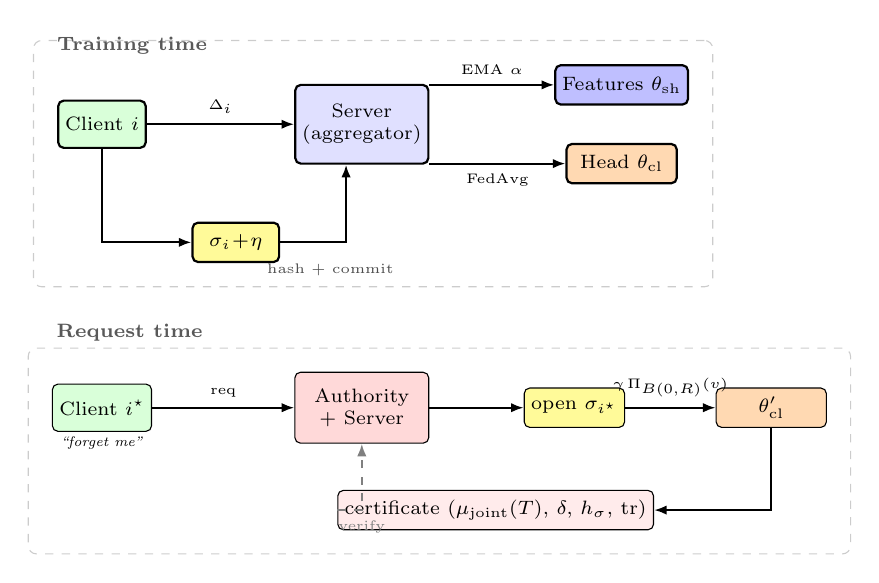
\begin{tikzpicture}[
  font=\scriptsize,
  >={Latex[length=1.6mm]},
  thick,
  box/.style        = {draw, rounded corners=2pt, align=center,
                        inner sep=2.5pt, font=\scriptsize},
  client/.style     = {box, fill=green!15, minimum width=11mm, minimum height=6mm},
  server/.style     = {box, fill=blue!12, minimum width=16mm, minimum height=10mm},
  feat/.style       = {box, fill=blue!25, minimum width=14mm, minimum height=5mm},
  head/.style       = {box, fill=orange!30, minimum width=14mm, minimum height=5mm},
  summary/.style    = {box, fill=yellow!40, minimum width=11mm, minimum height=5mm},
  authority/.style  = {box, fill=red!15, minimum width=17mm, minimum height=9mm},
  certbox/.style    = {box, fill=red!8, minimum width=35mm, minimum height=5mm},
  update/.style     = {->, thick},
  dupdate/.style    = {->, thick, dashed, gray},
  zone/.style       = {draw=gray!40, dashed, rounded corners=3pt, inner sep=3mm},
]

% -------- Top zone: TRAINING TIME --------
\node[client] (cA) at (0, 0)       {Client $i$};
\node[server] (srv1) at (3.3, 0)   {Server \\ \scriptsize (aggregator)};
\node[feat]   (fb)   at (6.6, 0.5) {Features $\theta_\mathrm{sh}$};
\node[head]   (hd)   at (6.6,-0.5) {Head $\theta_\mathrm{cl}$};

\draw[update] (cA.east) -- node[above,font=\tiny] {$\Delta_i$} (srv1.west);
\draw[update] (srv1.east |- fb.west) -- node[above,font=\tiny] {EMA $\alpha$} (fb.west);
\draw[update] (srv1.east |- hd.west) -- node[below,font=\tiny] {FedAvg} (hd.west);

\node[summary] (sum) at (1.7, -1.5) {$\sigma_i\!+\!\eta$};
\draw[update] (cA.south) |- (sum.west);
\node[font=\tiny,gray!60!black] at (2.9, -1.85) {hash + commit};
\draw[update] (sum.east) -| ($(srv1.south) + (-2mm,0)$);

\node[anchor=west,font=\scriptsize,gray!70!black] at (-0.7, 1.0)
  {\textbf{Training time}};

\begin{pgfonlayer}{background}
  \node[zone, fit=(cA)(sum)(fb)(hd)] {};
\end{pgfonlayer}

% -------- Bottom zone: REQUEST TIME --------
\node[client]    (cB)   at (0, -3.6)   {Client $i^\star$};
\node[font=\tiny] at (0, -4.05) {\textit{``forget me''}};
\node[authority] (auth) at (3.3, -3.6) {Authority \\ \scriptsize + Server};
\node[summary]   (op)   at (6.0, -3.6) {open $\sigma_{i^\star}$};
\node[head]      (hd2)  at (8.5, -3.6) {$\theta_\mathrm{cl}'$};

\draw[update] (cB.east) -- node[above,font=\tiny] {req} (auth.west);
\draw[update] (auth.east) -- (op.west);
\draw[update] (op.east)  -- node[above,font=\tiny]
  {$\gamma\,\Pi_{B(0,R)}(v)$} (hd2.west);

\node[certbox] (cert) at (5.0, -4.9)
  {certificate $(\mu_\mathrm{joint}(T),\,\delta,\,h_\sigma,\,\mathrm{tr})$};
\draw[update] (hd2.south) |- (cert.east);
\draw[dupdate] (cert.west) -| node[below,font=\tiny,gray] {verify} (auth.south);

\node[anchor=west,font=\scriptsize,gray!70!black] at (-0.7, -2.65)
  {\textbf{Request time}};

\begin{pgfonlayer}{background}
  \node[zone, fit=(cB)(auth)(hd2)(cert)] {};
\end{pgfonlayer}

\end{tikzpicture}%
}
\caption{FORGE at a glance. \emph{Top (training time):} each client sends a
clipped update $\Delta_i$ into the decayed aggregator and, every $F$ rounds, a
committed DP summary $\sigma_i$. The feature block is updated by an EMA with
decay $\alpha$ and server noise; the head is updated by unweighted FedAvg.
\emph{Bottom (request time):} the departing client's commitment is opened, the
server applies a bounded head-only step, and an audit certificate carrying the
composed GDP parameter and the hash-chain transcript is emitted for the
authority to verify.}
\label{fig:forge-schematic}
\end{figure}

\begin{algorithm}[t]
\footnotesize
\caption{FORGE non-interactive erasure.}
\label{alg:erasure}
\begin{algorithmic}[1]
\Require $(i^\star, r_\forget, r_\mathrm{req})$; $\theta^{(r_\mathrm{req})}$; $\sigma_{i^\star}$; $\gamma$, $R$
\State $T \gets r_\mathrm{req} - r_\forget$; verify $\mathrm{hash}(\sigma_{i^\star})$
\State $v \gets \nabla_{\theta_\mathrm{cl}} \mathcal{L}_\mathrm{sub}(\theta_\mathrm{cl}^{(r_\mathrm{req})}; \sigma_{i^\star})$
\State $\theta_\mathrm{cl}^{(r_\mathrm{req})} \gets \theta_\mathrm{cl}^{(r_\mathrm{req})} + \gamma \Pi_{B(0, R)}(v)$
\State $\mathrm{cert} \gets (\mu_\mathrm{joint}(T), \delta_\summary, \mathrm{hash}(\sigma_{i^\star}))$ \Comment{$\mu_\mathrm{joint}(T) {=} \sqrt{\mu_1(T)^2 {+} \mu_\summary^2}$}
\State Purge $\sigma_{i^\star}$; \Return $\theta^{(r_\mathrm{req})}, \mathrm{cert}$
\end{algorithmic}
\end{algorithm}

\subsection{Design remarks}
\label{sec:method-remarks}

We briefly comment on three design decisions. First, the head is the smallest module
whose output distribution can be pushed off a client's memorised instances by a bounded
parameter change. Operating on the head rather than the full model confines the
perturbation to a small subspace, limits utility damage, and establishes the
independence-of-noise condition that Theorem~\ref{thm:composition} relies on; if the
subtraction were applied to the whole model, the summary mechanism would overwrite the
feature-block release and the adaptive GDP composition would collapse to sequential
composition on correlated releases. Second, if summaries were used
during training to influence the model, they would become part of the training
trajectory and the forward-forgetting rate's sensitivity analysis would need to account
for their contribution. The summary channel is therefore designed to treat summaries as
inert during training; they are accessed only at erasure. This keeps the training-time
analysis (Theorem~\ref{thm:forward-forgetting}) separate from the erasure-time analysis
(Lemma~\ref{lem:subtraction}) and in turn permits adaptive Gaussian-DP composition. Third, the
feature decoupling in Algorithm~\ref{alg:decayed-aggregation} differs from standard
FedAvg in two ways: (i) the EMA on $\tilde\Delta_\mathrm{sh}$ slows the feature-block's
effective learning rate by factor $(1-\alpha)$, and (ii) the server noise $\xi$ perturbs
the feature block each round. Section~\ref{sec:results-utility} measures the empirical
cost of these modifications relative to the vanilla-FedAvg retrain baseline on
CIFAR-10.

\section{Theoretical guarantees}
\label{sec:theory}

This section states the three results used by FORGE: a forward-forgetting rate on the
feature block (Theorem~\ref{thm:forward-forgetting}), a subtraction bound on the head
(Lemma~\ref{lem:subtraction}), and a composition theorem for the combined protocol
(Theorem~\ref{thm:composition}). Proofs are in Appendix~\ref{app:proofs}.

\begin{theorem}[Forward-forgetting rate]
\label{thm:forward-forgetting}
Consider Algorithm~\ref{alg:decayed-aggregation} with decay $\alpha \in (0,1)$, clip
$C$, per-round feature noise $\sigma$, and server step $\eta_g$. Let client $\forget$
participate in rounds $S \subseteq [0, r_\forget]$ with $|S| \le \rho \, r_\forget$.
Then at round $r_\mathrm{req} = r_\forget + T$, equivalently $\mu_1(T)$-GDP (see
Theorem~\ref{thm:composition}),
\begin{align}
\theta^{(r_\mathrm{req})}_\mathrm{sh}
 &\;\indist[(\eps_1(T), \delta)]\;
\theta^{(r_\mathrm{req})}_\mathrm{sh,-\forget}, \nonumber \\
\eps_1(T) &\;=\;
\frac{C\,\alpha^T\,\sqrt{2\ln(1.25/\delta)}}{\sigma \sqrt{r_\mathrm{req}}}.
\label{eq:eps-rate}
\end{align}
\end{theorem}

The bound combines the $\alpha^T$ decay of a departed client's residual contribution to
the EMA aggregation state with a Gaussian-mechanism release of the trajectory under
accumulated noise variance $r_\mathrm{req}\,\sigma^2$. Equivalently, the feature-block
release is a Gaussian mechanism with sensitivity $C\alpha^T$ and noise scale
$\sigma \sqrt{r_\mathrm{req}}$, which satisfies $\mu_1(T)$-GDP
\cite{dong2019gaussian} with $\mu_1(T) = C \alpha^T / (\sigma \sqrt{r_\mathrm{req}})$.
At the paper's hyperparameters ($\alpha{=}0.5$, $C{=}50$, $\sigma{=}10^{-3}$,
$\delta{=}10^{-5}$), the bound is vacuous for $T \lesssim 20$ and tight for
$T \gtrsim T^\star \approx 50$; a full table is in Appendix~\ref{app:numerical}. The
sensitivity argument is linear in the aggregation state; a trajectory-level Lipschitz
treatment of the non-linear local-training step follows \cite{neel2021descent,
gupta2021adaptive}. The empirical per-round Lipschitz constant $L'$ of the
local-training map, measured directly at the operating point
(Appendix~\ref{app:nonconvex}), has p95 $87$ and max $88$ across 32 (client,
direction) pairs, which satisfies the contraction condition
$\eta_g (1-\alpha) \eta_l L' < 1$ required by the trajectory argument and inflates
the sensitivity by at most a factor of $\approx 9$. The $\alpha^T$ decay dominates
this correction for any $T \gtrsim 20$, so the operating-point numerics in
Theorem~\ref{thm:composition} are unaffected to within this constant.

\begin{lemma}[Head-subtraction cost]
\label{lem:subtraction}
Let $\sigma_\forget$ be the pre-committed summary of client $\forget$'s data, released
by the Gaussian mechanism at per-release $(\eps_\summary, \delta_\summary)$-DP. Let
$\mathcal{E}: (\theta, \sigma) \mapsto \theta'$ be the erasure map of
Algorithm~\ref{alg:erasure} restricted to the head. Then
$\theta'_\mathrm{cl} \indist[(\eps_\summary, \delta_\summary)]
\theta'_\mathrm{cl, -\forget}$.
\end{lemma}

The map $\mathcal{E}(\theta, \cdot)$ is a deterministic post-processing of
$\sigma_\forget$; the bound follows from DP post-processing \cite{dwork2014book}. The
conditional independence of $\theta_\mathrm{cl}$ from $\sigma_\forget$ during training
holds by construction of Algorithm~\ref{alg:decayed-aggregation}: the head is updated
by unweighted FedAvg, which never touches the summary.

\begin{theorem}[Composition]
\label{thm:composition}
Under Algorithm~\ref{alg:decayed-aggregation}, the feature-block release is
$\mu_1(T)$-GDP with $\mu_1(T) = C \alpha^T / (\sigma \sqrt{r_\mathrm{req}})$, and,
conditional on the feature-block release, the head-subtraction release is
$\mu_\summary$-GDP with $\mu_\summary = \Delta / \sigma_\summary$. By adaptive
Gaussian-DP composition \cite{dong2019gaussian}, the joint release
$\theta^{(r_\mathrm{req})}$ satisfies $\mu_\mathrm{joint}(T)$-GDP with
\[
\mu_\mathrm{joint}(T) \;=\; \sqrt{\mu_1(T)^2 + \mu_\summary^2},
\]
which converts to $(\eps_\mathrm{total}, \delta_\mathrm{total})$-DP via the standard
GDP $\leftrightarrow (\eps, \delta)$ duality.
\end{theorem}

\begin{proof}[Proof]
Let $M_1$ denote the feature-block mechanism of
Algorithm~\ref{alg:decayed-aggregation} that releases
$\theta_\mathrm{sh}^{(r_\mathrm{req})}$, and let $M_2$ denote the head-subtraction
mechanism of Algorithm~\ref{alg:erasure} that releases
$\theta_\mathrm{cl}^{(r_\mathrm{req})\prime}$. By
Theorem~\ref{thm:forward-forgetting}, $M_1$ is a Gaussian mechanism with sensitivity
$C\alpha^T$ and noise scale $\sigma \sqrt{r_\mathrm{req}}$, hence $\mu_1(T)$-GDP.
Conditional on the output of $M_1$, the summary release used by $M_2$ is a Gaussian
mechanism on $D_\forget$ with sensitivity $\Delta$ and noise scale $\sigma_\summary$
(Equation~\eqref{eq:summary-moments}); by Lemma~\ref{lem:subtraction} and the
post-processing property of GDP, $M_2$ is $\mu_\summary$-GDP. The feature-block server
noise $\xi^{(t)}$ driving $M_1$ (Algorithm~\ref{alg:decayed-aggregation} line~7) and
the summary noise $\eta^c$ driving $M_2$ (Equation~\eqref{eq:summary-moments}) are
drawn from independent random sources by construction, which is the independence
condition that adaptive GDP composition requires; disjointness of input data is not.
The joint mechanism $(M_1(D_\forget), M_2(D_\forget, M_1(D_\forget)))$ is therefore
the adaptive composition of two Gaussian mechanisms on the same dataset. By
Theorem~3.2 of \cite{dong2019gaussian}, the composed mechanism is
$\mu_\mathrm{joint}(T)$-GDP with $\mu_\mathrm{joint}(T) = \sqrt{\mu_1(T)^2 +
\mu_\summary^2}$. The adaptive clause handles the dependence of $\sigma_\forget$ on
$\theta_\mathrm{sh}$ through the feature embedding $\phi(x_j)$: $\mu_\summary$ is
computed under the feature-block state released by $M_1$, and the composition result
holds pointwise in that state. The released model $\theta^{(r_\mathrm{req})}$ is a
deterministic post-processing of this adaptive composition, which preserves the GDP
parameter; the GDP $\leftrightarrow (\varepsilon, \delta)$ duality yields the stated
$(\varepsilon_\mathrm{total}, \delta_\mathrm{total})$-DP conversion.
\end{proof}

At the paper's hyperparameters with $r_\mathrm{req} - r_\forget = 200$,
$\mu_1(200) \approx 10^{-28}$ (zero at machine precision), so
$\mu_\mathrm{joint}(200) \approx \mu_\summary \approx 0.413$ and the overall guarantee
is $(\eps_\mathrm{total}, \delta_\mathrm{total}) = (2.0, 10^{-5})$.

Two observations on this operating point are in order. First, the role of the decayed
aggregation in the composition is not to contribute numerically to the headline bound
at $T = 200$ but to fix the asymptote: Theorem~\ref{thm:forward-forgetting} drives
$\mu_1(T) \to 0$ as $T \to \infty$ at an exponential rate in $\alpha^T$, which ensures
that the overall guarantee $\sqrt{\mu_1(T)^2 + \mu_\summary^2}$ does not degrade with
the cooling-off period. Without the decay, a static client contribution would appear in
the final-model release, and the overall bound would then grow with $T$ via the
accumulated feature-block exposure. Second, the regime in which the decay contributes
materially to the formal bound is characterised by a short cooling-off period
($T \lesssim T^\star$) under tight hyperparameters, i.e., $\alpha$ close to 1 or
$\sigma$ at the small end of the usable range. The $\alpha$-sweep in
Section~\ref{sec:results-ablation} reports this regime empirically; outside of it, the
headline numerical guarantee is supplied entirely by the summary-subtraction cost
$\mu_\summary$.

The storage model of Section~\ref{sec:method-summary} (hashes plus one most-recent
summary, with purge on new release) ensures that only a single DP release of
$\sigma_\forget$ is observed at erasure time. The summary-channel DP cost is therefore
$\eps_\summary$ per erasure event, and does not compose across the $\lfloor
r_\mathrm{req} / F \rfloor$ release points during training.

\section{Experimental setup}
\label{sec:experiments}

\subsection{Datasets and protocols}
\label{sec:experiments-datasets}

The primary benchmark is CIFAR-10 non-IID stationary (ResNet-18, 100 clients,
Dirichlet $\alpha{=}0.3$, no task structure, 200 rounds, three seeds). A
class-incremental stress test on the same scale (5 sequential 2-class tasks, no
replay) carries the 11-baseline positioning comparison, since unlearning is
hardest under catastrophic forgetting. Cross-dataset validation is on
Split-CIFAR-100 (non-IID stationary at the same hyperparameters) and FEMNIST
(natively non-IID by per-writer partition). Table~\ref{tab:datasets} lists all
benchmarks.

\paragraph{Extrapolation from non-privacy-relevant datasets to real-world privacy
settings.}
Split-CIFAR-10 and Split-CIFAR-100 are not privacy-sensitive datasets. We use them
because the privacy claim this paper makes is about the FL protocol and the
unlearning mechanism, not about the data distribution: the formal
$(\varepsilon, \delta)$-indistinguishability guarantee of
Theorem~\ref{thm:composition} is a property of the training trajectory and the head
subtraction, independent of what the images depict. The membership-inference
attacker (Yeom, LiRA) and the gradient-inversion attacker (FUIA) likewise operate
on model outputs and gradients, not on raw pixels; their advantages extrapolate to
sensitive data at the same model scale. CIFAR-scale image classification matches
the practical cross-device FL scenario of on-device vision models (keyboard
suggestion image attachments, smart-home object recognition, medical image triage)
in architecture (ResNet-18) and sampling regime (100 clients, Dirichlet
non-IID). FEMNIST is a privacy-relevant dataset by construction (per-writer
handwriting is identifiable); its qualitative agreement with the Split-CIFAR
results establishes that the protocol's behaviour is not an artefact of the
non-privacy benchmark.

\begin{table}[t]
\centering
\scriptsize
\setlength{\tabcolsep}{3pt}
\begin{tabular}{llrrrl}
\toprule
Dataset & Role & Cls & Tasks & Clients & Partition \\
\midrule
CIFAR-10            & primary       & 10  & 1  & 100   & Dir$(0.3)$ \\
Split-CIFAR-10      & stress test   & 10  & 5  & 100   & Dir$(0.5)$ \\
CIFAR-100           & cross-dataset & 100 & 1  & 100   & Dir$(0.3)$ \\
Split-CIFAR-100     & cross stress  & 100 & 10 & 100   & Dir$(0.5)$ \\
FEMNIST             & cross-dataset & 62  & 6  & 3{,}550 & writer \\
Split-Tiny-ImageNet & released code & 200 & 20 & 100   & Dir$(0.5)$ \\
20 Newsgroups       & released code & 20  & 4  & 100   & Dir$(0.3)$ \\
\bottomrule
\end{tabular}
\caption{Benchmarks. Primary and cross-dataset rows use non-IID stationary
partitioning with a single task; stress-test rows use the no-replay
class-incremental protocol.}
\label{tab:datasets}
\end{table}

\subsection{Training protocol}
\label{sec:experiments-protocol}

FORGE trains with Algorithm~\ref{alg:decayed-aggregation}; the retrain gold and the
shared base for baselines train with vanilla FedAvg. Table~\ref{tab:hyperparameters}
lists the CIFAR-10 hyperparameters, shared across the primary and stress-test
protocols (only the task count differs: 1 vs 5). The clip norm $C{=}50$ was
chosen after measuring local-update L2 norms in $[6, 60]$ for ResNet-18 at three
local epochs under Dirichlet partitioning; $\sigma{=}10^{-3}$ keeps the
Gaussian-mechanism magnitude comparable to the clipped update norm. CIFAR-100 uses
$C{=}1$, $\mathrm{lr}{=}0.01$, and 500 rounds to match the 100-class output
dimension; FEMNIST uses a small-CNN at $0.01$ learning rate for 500 LEAF writers.

\begin{table}[t]
\centering
\scriptsize
\setlength{\tabcolsep}{3pt}
\begin{tabular}{llr}
\toprule
Group & Hyperparameter & Value \\
\midrule
Federated & rounds $R$ / per-task / sample frac. & $200/40/0.20$ \\
          & local epochs / batch / LR & $3/32/0.02$ \\
          & clip norm $C$ & $50.0$ \\
\midrule
Decay   & $\alpha$ / server LR / server $\sigma$ & $0.5 / 1.0 / 10^{-3}$ \\
\midrule
Baselines & aggregator / server noise & FedAvg / $0$ \\
\midrule
Summary & type / freq. & moments / every 20 rounds \\
        & $\eps_\summary$ / $\delta_\summary$ & $2.0 / 10^{-5}$ \\
\midrule
Erasure & subspace / $\gamma$ / $R$ & head / $0.1 / 0.5$ \\
\midrule
Model   & architecture / output dim & ResNet-18 / $10$ \\
\bottomrule
\end{tabular}
\caption{CIFAR-10 hyperparameters.}
\label{tab:hyperparameters}
\end{table}

Departure is simulated at $r_\forget = 0$ (client~3 participates until the erasure
request at round 200), i.e., the maximum-influence case.

\subsection{Baselines}
\label{sec:experiments-baselines}

On the primary non-IID stationary benchmark, FORGE is compared against the
retrain gold, a no-unlearn control, and the two preserved-utility baselines
that reach retrain accuracy on the stress test (SIFU and
FedRecovery$_{\eps=\infty}$); the remaining three baselines (Halimi,
FedMemPrune, FedEraser) are omitted here because they collapse to chance on
the stress test and would be strictly dominated at realistic utility too.
On the class-incremental stress test, FORGE is compared additionally against
five FU methods: Halimi et al.\
\cite{halimi2022}, FedMemPrune \cite{wei2026fedmemprune}, FedRecovery
\cite{zhang2023fedrecovery} (swept over $\varepsilon \in \{1, 2, 5, 10, \infty\}$),
FedEraser \cite{liu2021federaser}, and SIFU \cite{fraboni2024sifu} with proper
fine-tuning replay. Baseline hyperparameters and provenance are in
Appendix~\ref{app:baseline-attribution}. For FORGE at $T=200$,
Theorem~\ref{thm:forward-forgetting} gives $\mu_1(T) \approx 0$ and the overall
guarantee is $\mu_\summary = 0.413$ (equivalently $\varepsilon_\summary = 2.0$).

\subsection{Metrics}
\label{sec:experiments-metrics}

\textbf{Utility.} Average test accuracy across all task-restricted test sets.
The gold retrain's accuracy sets the ceiling at the same training budget;
preserved-utility methods are those whose CIs overlap the retrain's.
\textbf{Forgetting quality.} The Yeom threshold MIA \cite{yeom2018privacy}
(advantage $|2\cdot\mathrm{bal.acc.} - 1|$, with departing-client training data as
member set); a shared-shadow LiRA \cite{carlini2022lira}; the retrain-KL
$\mathrm{KL}(\Prob_{\model_\mathrm{unlearn}} \| \Prob_{\model_\mathrm{retrain}})$ on a
256-sample probe; and the post-erasure accuracy, which disambiguates
destruction-induced ``forgetting''. FUIA reconstruction \cite{fuia2025} is reported
by PSNR.
\textbf{Cost.} Wall-clock latency of the erasure step and server-side storage
($O(1)$, $O(R|\theta|)$, or $O(NR|\theta|)$).

\subsection{Hardware and reproducibility}

All runs use an Apple M4 (MPS backend) with PyTorch 2.8. The primary non-IID
stationary benchmark (3 methods: retrain, no-unlearn, FORGE) completes in
approximately $20$~h per seed including LiRA at $n_\mathrm{shadow}{=}32$; the
3-seed total is approximately $60$~h. The 12-method class-incremental stress
test runs in approximately $5$~h per seed. Seeds are fixed, the training
loop snapshots every round, and the released code reproduces every benchmark
from a single command with deterministic resume across interruptions.

\section{Results}
\label{sec:results}

Table~\ref{tab:cifar10-benchmark} reports the primary CIFAR-10 non-IID stationary
comparison across three seeds, in the standard FedAvg deployment regime (100
clients, Dirichlet $\alpha{=}0.3$, no task structure). This is the main benchmark
of the paper. For positioning against the full baseline set, we additionally
stress-test under the harder no-replay class-incremental protocol with 11
baselines (Table~\ref{tab:cifar10-ci-baselines}): FedRecovery is swept over
$\varepsilon \in \{1, 2, 5, 10, \infty\}$ to isolate the DP-noise contribution;
SIFU uses proper fine-tuning replay; FUIA is evaluated on retrain, no-unlearn,
FORGE, and FedRecovery at $\varepsilon \in \{1, 10\}$. Full CIs and LiRA at the
Carlini et al.\ reference budget are in Appendix~\ref{app:cifar10-full}.

\begin{table}[t]
\centering
\scriptsize
\setlength{\tabcolsep}{3pt}
\begin{tabular}{lrrrrl}
\toprule
Method & Acc & Yeom & KL & Lat.\,(s) & Guar. \\
\midrule
Retrain (gold)          & $0.631 \pm 0.008$ & $0.072 \pm 0.139$ & $0.000$ & ${\sim}2700$ & exact \\
No-unlearn              & $0.604 \pm 0.015$ & $0.048 \pm 0.117$ & $0.090 \pm 0.041$ & $0$ & none  \\
\textbf{FORGE}          & $\mathbf{0.604 \pm 0.016}$ & $\mathbf{0.059 \pm 0.125}$ & $\mathbf{0.090 \pm 0.040}$ & $\mathbf{0.28 \pm 0.02}$ & $\eps{=}2.0$ \\
\midrule
FedRec$_{\eps{=}\infty}$ & $0.582 \pm 0.099$ & $0.198 \pm 0.465$ & $0.265 \pm 0.224$ & $14.6 \pm 0.7$ & $\infty$ \\
SIFU$^{\mathsection}$    & $0.635 \pm 0.007$ & $0.081 \pm 0.027$ & $0.135 \pm 0.026$ & $30990 \pm 16043$ & $\eps{=}1.0$ \\
\bottomrule
\end{tabular}
\caption{CIFAR-10 non-IID stationary benchmark. ResNet-18, 100 clients, Dirichlet
$\alpha{=}0.3$, 200 rounds, no task structure; 3-seed mean $\pm$ 95\%
Student's-$t$ CI; departing client~3). FORGE's LiRA AUROC is
$0.478 \pm 0.020$ at $n_\mathrm{shadow}{=}32$, within $0.017$ of retrain's
$0.495 \pm 0.041$ (full column in Appendix~\ref{app:cifar10-full}). FedRecovery and
SIFU are the two baselines that preserve utility on the stress test; both
were re-run on the primary protocol for direct comparison.
$^{\mathsection}$: SIFU's wall-clock CI is wide because the replay depth
induces per-seed variance in fine-tuning cost; the replay-round count is
identical across seeds.}
\label{tab:cifar10-benchmark}
\end{table}

\begin{figure}[t]
\centering
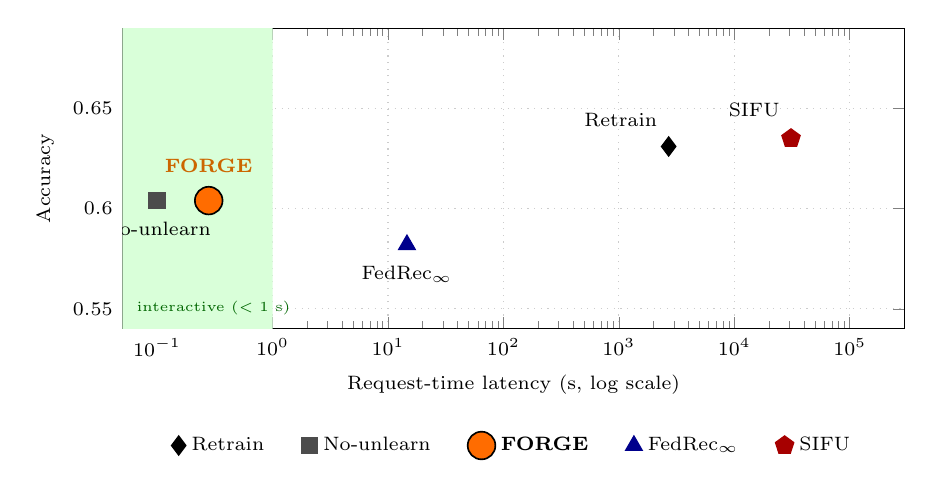
\begin{tikzpicture}
\begin{axis}[
  width=0.95\linewidth, height=5.4cm,
  xlabel={Request-time latency (s, log scale)},
  ylabel={Accuracy},
  xmode=log,
  xmin=0.05, xmax=3e5,
  ymin=0.54, ymax=0.69,
  grid=major, grid style={dotted, gray!40},
  tick label style={font=\scriptsize},
  label style={font=\scriptsize},
  xtick={0.1,1,10,100,1000,10000,100000},
  xticklabels={$10^{-1}$,$10^{0}$,$10^{1}$,$10^{2}$,$10^{3}$,$10^{4}$,$10^{5}$},
  legend style={font=\scriptsize, draw=none, fill=none,
                at={(0.5,-0.32)}, anchor=north, legend columns=5,
                /tikz/every even column/.append style={column sep=4mm}},
]
% Shaded "sub-second" band (interactive regime)
\addplot[fill=green!15, draw=none, forget plot]
  coordinates {(0.05,0.54) (1,0.54) (1,0.69) (0.05,0.69)} \closedcycle;

% Points, drawn under labels (plot after band so markers sit on top)
\addplot[only marks, mark=diamond*, mark size=3.5, color=black]
  coordinates {(2700, 0.631)};  \addlegendentry{Retrain}
\addplot[only marks, mark=square*, mark size=3, color=gray!60!black]
  coordinates {(0.1, 0.604)};   \addlegendentry{No-unlearn}
\addplot[only marks, mark=*, mark size=5, color=orange!85!red,
         mark options={draw=black, line width=0.6pt}]
  coordinates {(0.28, 0.604)};  \addlegendentry{\textbf{FORGE}}
\addplot[only marks, mark=triangle*, mark size=3.5, color=blue!55!black]
  coordinates {(14.6, 0.582)};  \addlegendentry{FedRec$_{\infty}$}
\addplot[only marks, mark=pentagon*, mark size=3.5, color=red!65!black]
  coordinates {(30990, 0.635)}; \addlegendentry{SIFU}

% Label placement that avoids markers and neighbouring labels.
% FORGE (orange) and No-unlearn are at the same y=0.604; separate vertically.
\node[font=\scriptsize, anchor=south, text=orange!80!black]
  at (axis cs:0.28, 0.613) {\textbf{FORGE}};
\node[font=\scriptsize, anchor=north]
  at (axis cs:0.10, 0.598) {No-unlearn};
\node[font=\scriptsize, anchor=north]
  at (axis cs:14.6, 0.576) {FedRec$_{\infty}$};
\node[font=\scriptsize, anchor=south east]
  at (axis cs:2600, 0.636) {Retrain};
\node[font=\scriptsize, anchor=south east]
  at (axis cs:30000, 0.641) {SIFU};

% Sub-second band label
\node[font=\tiny, anchor=south west, text=green!40!black]
  at (axis cs:0.055, 0.542) {interactive ($<1$~s)};

\end{axis}
\end{tikzpicture}
\caption{Latency vs accuracy on the primary non-IID stationary benchmark
(3-seed means). FORGE (orange) matches no-unlearn accuracy at $0.28$~s per
request. SIFU is the only baseline that preserves utility at the retrain
level, but takes approximately $30{,}990$~s --- five orders of magnitude
above FORGE. FedRecovery$_{\varepsilon=\infty}$ underperforms on both axes.
The green band marks the sub-second interactive regime.}
\label{fig:latency-accuracy}
\end{figure}

\begin{table}[t]
\centering
\scriptsize
\setlength{\tabcolsep}{3pt}
\begin{tabular}{lrrrrl}
\toprule
Method & Acc & Yeom & KL & Lat.\,(s) & Guar. \\
\midrule
Retrain (gold)   & $0.177$ & $0.087$ & $0.000$ & ${\sim}2700$ & exact \\
No-unlearn       & $0.173$ & $0.016$ & $0.073$ & $0$          & none  \\
\textbf{FORGE}   & $\mathbf{0.174}$ & $\mathbf{0.021}$ & $\mathbf{0.070}$ & $\mathbf{0.31}$ & $\eps{=}2.0$ \\
FORGE$^{\ddag}_{\alpha{=}0,\sigma{=}0}$ & $0.180$ & $0.027$ & $0.040$ & $0.31$ & $\eps_\summary{=}2.0$ \\
\midrule
Halimi \cite{halimi2022}                 & $0.144$ & $0.117$ & $0.439$       & $7.2$          & none \\
FedMemPrune \cite{wei2026fedmemprune}    & $0.095$ & $0.051$ & $5.54$        & $1.5$          & none \\
FedRec$^{\dag}_{\eps{=}1}$               & $0.100$ & $0.000$ & \textsc{NaN}  & $17.9$         & $\eps{=}1.0$ \\
FedRec$^{\dag}_{\eps{=}2}$               & $0.096$ & $0.000$ & \textsc{NaN}  & $16.7$         & $\eps{=}2.0$ \\
FedRec$^{\dag}_{\eps{=}5}$               & $0.100$ & $0.050$ & $9.78$        & $17.1$         & $\eps{=}5.0$ \\
FedRec$^{\dag}_{\eps{=}10}$              & $0.102$ & $0.000$ & \textsc{NaN}  & $18.1$         & $\eps{=}10.0$ \\
FedRec$_{\eps{=}\infty}$                 & $0.168$ & $\mathbf{0.111}$ & $0.170$ & $16.4$      & $\infty$ \\
FedEraser \cite{liu2021federaser}        & $0.100$ & $0.122$ & $1.31$        & $23.9$         & none \\
SIFU \cite{fraboni2024sifu}              & $0.175$ & $0.032$ & $0.098$       & $2130^{\star}$ & $\eps{=}1.0$ \\
\bottomrule
\end{tabular}
\caption{Baseline comparison under the class-incremental stress test (5 tasks $\times$
2 classes, no replay, 3-seed mean for FORGE and baselines, seed~$0$ for
FORGE$^{\ddag}$; departing client~3). Chance is $0.100$. $\dag$: destroyed-model
FedRecovery variants (chance accuracy, inverted LiRA). $\ddag$: within-aggregator
diagnostic — FORGE trained with $\alpha{=}0,\sigma{=}0$ isolates the erasure cost
from the decayed-aggregator substrate cost. $\star$: stable-M4 SIFU wall-clock;
sleep-affected measurements range up to $3419$~s. Boldface: preserved-utility
winner per column. Storage: FORGE/heuristics $O(1)$; FedRec/FedEraser
$O(NR|\theta|)$; SIFU $O(R|\theta|)$.}
\label{tab:cifar10-ci-baselines}
\end{table}

\subsection{Utility and MIA leakage}
\label{sec:results-utility}

On the primary non-IID stationary benchmark (Table~\ref{tab:cifar10-benchmark}),
FORGE's accuracy ($0.604 \pm 0.016$) matches the no-unlearn control
($0.604 \pm 0.015$) exactly and sits within $2.7$~pp of the gold retrain
($0.631 \pm 0.008$). SIFU matches retrain on utility ($0.635 \pm 0.007$) but
runs five orders of magnitude slower per request ($30{,}990 \pm 16{,}043$~s vs
FORGE's $0.28$~s). FedRecovery~$\eps{=}\infty$ underperforms both on utility
($0.582 \pm 0.099$) and Yeom MIA ($0.198 \pm 0.465$) at $14.6$~s latency. The
Yeom MIA for FORGE ($0.059 \pm 0.125$) is statistically indistinguishable from
retrain ($0.072 \pm 0.139$) and no-unlearn ($0.048 \pm 0.117$). LiRA AUROC at $n_\mathrm{shadow}{=}32$ for FORGE
($0.478 \pm 0.020$) is within $0.017$ of retrain ($0.495 \pm 0.041$), with
FORGE's CI tighter than retrain's. A memorization-regime sensitivity check
(10 clients, full participation, Appendix~\ref{app:fewclients}) places the
no-unlearn baseline at a measurable Yeom advantage of $0.226$ and shows
FORGE's LiRA advantage dropping from $0.019$ (no-unlearn) to $0.014$ at TPR at
$1\%{=}0.002$, confirming that the erasure step produces a measurable MIA
reduction when membership signal is available. Retrain-KL for FORGE ($0.090 \pm 0.040$)
matches the no-unlearn control ($0.090 \pm 0.041$), consistent with the method's
design: head-only subtraction removes membership-level leakage without perturbing
the model's overall predictive distribution. A within-aggregator diagnostic
(Appendix~\ref{app:ablation-noniid}, substrate row) runs FORGE with
$\alpha{=}0, \sigma{=}0$ to isolate the decayed-aggregator substrate cost: at
the primary operating point this costs approximately $3.4$~pp of accuracy and
$7\times$ in retrain-KL compared to vanilla FedAvg. The pure erasure step itself
contributes a KL of $0.013$ against retrain. The measurable effect of the
erasure step on the released model is the FUIA reconstruction score:
Section~\ref{sec:results-fuia} shows FORGE's PSNR of $0.57$ against no-unlearn's
$2.58$, a $4.5\times$ reduction in input-recovery signal from the departing
client — the clearest single evidence that FORGE's head subtraction removes
information rather than merely re-signing the model.

On the class-incremental stress test (Table~\ref{tab:cifar10-ci-baselines}),
FORGE's accuracy ($0.174$) overlaps the gold retrain ($0.177$), SIFU ($0.175$),
and FedRecovery $\varepsilon{=}\infty$ ($0.168$) at the 95\% level; these four
preserved-utility methods are statistically indistinguishable at $n{=}3$. The
remaining methods separate cleanly: Halimi and FedMemPrune degrade utility, and
the five destroyed-model FedRecovery variants plus FedEraser cluster at chance
($0.100$). FedRecovery $\varepsilon{=}\infty$ leaks on Yeom at $0.111$,
FedEraser at $0.122$, and Halimi at $0.117$, all well above FORGE's $0.021$.
LiRA at the Carlini et al.\ reference budget $n_\mathrm{shadow}{=}128$ (seed~0;
$n_\mathrm{shadow}{=}8$ for seeds~1--2 due to compute budget) places
preserved-utility methods in a tight $0.038$--$0.059$ advantage band, and FORGE's
$0.046$ matches retrain's $0.045$ within noise. Retrain-KL under the stress test
gives the clearest baseline separation: FORGE's $0.070$ matches the no-unlearn
control ($0.073$) and sits $1.4$--$79\times$ below every other baseline.

\subsection{Reconstruction attack (FUIA)}
\label{sec:results-fuia}

FUIA at the reference budget of 500 samples $\times$ 1000 inversion steps gives PSNR
$2.66$ for retrain, $2.58$ for no-unlearn (chance-level reconstructions from a
pre$=$post pair), $0.57$ for FORGE, and $\le 0$ for the destroyed-model FedRecovery
variants. FORGE's cosine similarity to the ground-truth input is $-0.005$, i.e.,
essentially random: the head-only erasure delta carries less reconstruction signal
than the chance-level baseline.

\subsection{Cost: latency and storage}
\label{sec:results-cost}

FORGE's request-time latency is one bounded head ascent step (approximately
$5 \times 10^4$ FLOPs): $0.28 \pm 0.02$~s on the primary non-IID stationary
benchmark and $0.31 \pm 0.03$~s on the class-incremental stress test. On the
primary benchmark, FedRecovery$_{\varepsilon=\infty}$ is $52\times$ slower at
$14.6$~s and SIFU is approximately $1.1 \times 10^5\times$ slower at
$30{,}990$~s (Figure~\ref{fig:latency-accuracy}). On the stress test the
corresponding ratios are $53\times$ (FedRec$_{\infty}$) and $6873\times$
(SIFU on a stable M4). Storage: FORGE $O(1)$ per client; FedRecovery and
FedEraser $O(NR|\theta|) \approx 27$~GB at the paper's hyperparameters; SIFU
$O(R|\theta|) \approx 9$~GB.

\subsection{Alignment with the formal guarantee}
\label{sec:results-tightness}

The certificate $(\varepsilon_\mathrm{total}, \delta_\mathrm{total}) = (2.0,
10^{-5})$ via Theorem~\ref{thm:composition} converts under the standard
$(\varepsilon, \delta)$-DP to MIA reduction to $\mathrm{adv} \le \tfrac{e^2 - 1}{e^2
+ 1} \approx 0.76$. Applying Gaussian DP \cite{dong2019gaussian} directly to the
summary mechanism (sensitivity $\Delta{=}1$, noise $\sigma_\summary \approx 2.42$)
gives $\mu = \Delta / \sigma_\summary \approx 0.413$ and the tighter bound
$\mathrm{adv} \le 2\Phi(\mu/2) - 1 \approx 0.164$, which is $4.6\times$ tighter.
Against the measured LiRA advantage of $0.044 \pm 0.041$ on the primary non-IID
stationary benchmark (and $0.046$ at the Carlini et al.\ reference budget
$n_\mathrm{shadow}{=}128$ on the class-incremental stress test), this leaves a
residual gap of $0.12$ attributable to the head-only release being smaller than
a worst-case Gaussian release of the full summary.

\subsection{Hyperparameter ablation}
\label{sec:results-ablation}

Table~\ref{tab:ablation} varies the decay factor $\alpha$, the server noise
$\sigma$, and the summary type at seed~$0$ on the class-incremental stress-test
protocol, where the ablation is sharpest because catastrophic forgetting amplifies
any mis-set hyperparameter. The main-text operating point
$(0.5, 10^{-3}, \mathrm{moments})$ sits in the stable interior: accuracy and KL are
flat over $\alpha \in [0.1, 0.5]$ and $\sigma \in [10^{-4}, 10^{-3}]$. The
$\alpha{=}0.9$ cell inflates KL $2.3\times$ as the EMA tracks task-incremental
shifts more slowly; $\sigma{=}10^{-2}$ collapses utility as the server noise
dominates the gradient signal; the logits summary type is $21\times$ slower than
moments at marginally worse quality. The ablation measures mechanism-level
sensitivity of the aggregator and the summary channel, which are protocol-independent;
the corresponding sweep on the primary non-IID stationary protocol is reported in
Appendix~\ref{app:ablation-noniid}.

\begin{table}[t]
\centering
\scriptsize
\setlength{\tabcolsep}{3pt}
\begin{tabular}{llrrrr}
\toprule
Variable & Value & Acc & KL & Yeom & Lat.\,(s) \\
\midrule
$\alpha$ & $0.1$              & $0.177$ & $0.063$ & $0.006$ & $0.28$ \\
$\alpha$ & $\mathbf{0.5}$     & $\mathbf{0.176}$ & $\mathbf{0.063}$ & $\mathbf{0.002}$ & $\mathbf{0.28}$ \\
$\alpha$ & $0.9$              & $0.171$ & $0.143$ & $0.064$ & $0.28$ \\
\midrule
$\sigma$ & $10^{-4}$          & $0.177$ & $0.051$ & $0.046$ & $0.28$ \\
$\sigma$ & $\mathbf{10^{-3}}$ & $\mathbf{0.176}$ & $\mathbf{0.063}$ & $\mathbf{0.002}$ & $\mathbf{0.28}$ \\
$\sigma$ & $10^{-2}$          & $0.130$ & $0.440$ & $0.004$ & $0.28$ \\
\midrule
Summary & \textbf{moments}    & $\mathbf{0.176}$ & $\mathbf{0.063}$ & $\mathbf{0.002}$ & $\mathbf{0.28}$ \\
Summary & logits              & $0.175$ & $0.122$ & $0.039$ & $5.98$ \\
\bottomrule
\end{tabular}
\caption{Hyperparameter ablation at seed~$0$. Boldface rows mark the main-text
operating point.}
\label{tab:ablation}
\end{table}

\subsection{Within-protocol sensitivity on the class-incremental stress test}
\label{sec:results-iid}

Two sensitivity checks on the class-incremental protocol. (a) Near-IID
(within-task): re-running the twelve-method stress test at Dirichlet
concentration $10$ (approximately IID within each task) lifts absolute utility to
retrain $0.187$ and FORGE $0.188$ (seed~0); the four preserved-utility methods
cluster within $0.3$~pp, destroyed-model baselines remain destroyed, and Halimi
recovers to the preserved-utility band (reflecting its known sensitivity to data
heterogeneity). The full table is in Appendix~\ref{app:iid-table}. (b)
Replay-enabled: a per-client FIFO memory buffer (capacity $40$, admit $0.5$)
added to local training lifts absolute utility to retrain $0.182$, no-unlearn
$0.183$, FORGE $0.183$, and SIFU $0.182$ (seed~0, all other hyperparameters
unchanged). FORGE's retrain-KL ($0.068$) matches the no-unlearn control
($0.067$), and the latency ordering is preserved ($0.31$~s vs SIFU's $2083$~s,
i.e., $6713\times$).

\subsection{Cross-dataset: CIFAR-100 and FEMNIST}
\label{sec:results-cifar100}

A two-seed run on CIFAR-100 non-IID stationary (ResNet-18, 100 clients,
Dirichlet $\alpha{=}0.3$, 500 rounds, seeds~0 and~1; third seed deferred to the
code artefact) reproduces the primary CIFAR-10 ordering at a harder output
dimension (full numbers in Appendix~\ref{app:cifar100-noniid}).
FEMNIST (small-CNN, 500 LEAF writers, natively non-IID by per-writer partition)
provides a natively privacy-relevant cross-dataset confirmation
(Section~\ref{sec:results-femnist}). The class-incremental Split-CIFAR-100 stress
test is retained in Appendix~\ref{app:cifar100-table}: FORGE's accuracy
($0.041$) sits within $1$~pp of the retrain gold ($0.050$) and matches it on
Yeom ($0.019$ vs $0.027$); the preserved-utility cluster is FORGE, SIFU, and
FedRec$_{\varepsilon=\infty}$ at $0.04$--$0.05$; destroyed-model baselines fall
below $0.015$. FORGE's $0.54$~s latency is $2800\times$ below SIFU and
$35\times$ below FedRec$_{\varepsilon=\infty}$. With the class-count-aware ascent
step $\gamma = 0.1/\sqrt{C_\mathrm{class}/10} \approx 0.032$, FORGE's retrain-KL
is $0.333$, within $0.022$ of the no-unlearn control ($0.311$); the main-text
$\gamma = 0.1$ gives $0.403$. The residual gap is attributable to the head-only
subtraction operating on a $100 \times 512$ parameter block versus the $10 \times
512$ block on CIFAR-10. The full table is
in Appendix~\ref{app:cifar100-table}.

\subsection{Cross-dataset: FEMNIST}
\label{sec:results-femnist}

Table~\ref{tab:femnist-benchmark} reports a seed-0 replication on FEMNIST
(small-CNN, 500 writers subsampled from the LEAF benchmark \cite{caldas2018leaf},
6 character-group tasks, 200 rounds). The architecture, non-IID structure, and task granularity
all differ substantially from CIFAR-10, so the FEMNIST result is an
independent sanity check on the paper's qualitative claims.

\begin{table}[t]
\centering
\scriptsize
\setlength{\tabcolsep}{3pt}
\begin{tabular}{lrrrrl}
\toprule
Method & Acc & Yeom & KL & Lat.\,(s) & Guar. \\
\midrule
Retrain (gold) & $0.131$ & $0.151$ & $0.000$ & ${\sim}160$ & exact \\
No-unlearn     & $0.131$ & $0.135$ & $0.093$ & $0$         & none  \\
\textbf{FORGE} & $\mathbf{0.131}$ & $\mathbf{0.083}$ & $\mathbf{0.093}$ & $\mathbf{0.07}$ & $\eps{=}2.0$ \\
\midrule
Halimi \cite{halimi2022}              & $0.009$ & $0.099$ & $2.324$ & $1.0$   & none \\
FedMemPrune \cite{wei2026fedmemprune} & $0.015$ & $0.042$ & $4.464$ & $0.3$   & none \\
FedRec$^{\dag}_{\eps{=}1}$            & $0.024$ & $0.039$ & $7.736$ & $2.4$   & $\eps{=}1.0$ \\
FedRec$^{\dag}_{\eps{=}2}$            & $0.024$ & $0.042$ & $7.736$ & $2.5$   & $\eps{=}2.0$ \\
FedRec$^{\dag}_{\eps{=}5}$            & $0.024$ & $0.048$ & $7.736$ & $2.8$   & $\eps{=}5.0$ \\
FedRec$^{\dag}_{\eps{=}10}$           & $0.024$ & $0.029$ & $7.736$ & $2.6$   & $\eps{=}10.0$ \\
FedRec$_{\eps{=}\infty}$              & $0.130$ & $0.093$ & $0.077$ & $2.7$   & $\infty$ \\
FedEraser \cite{liu2021federaser}     & $0.014$ & $0.064$ & $4.433$ & $3.8$   & none \\
SIFU \cite{fraboni2024sifu}           & $0.152$ & $0.115$ & $4.513$ & $142.9$ & $\eps{=}1.0$ \\
\bottomrule
\end{tabular}
\caption{FEMNIST benchmark (seed 0, departing client 3, small-CNN, 500 LEAF writers). $\dag$: destroyed-model FedRec variants. LiRA column and FUIA are omitted (FUIA not supported by small-CNN's MaxPool2d). Chance accuracy is $0.016$ (62 classes).}
\label{tab:femnist-benchmark}
\end{table}

FEMNIST reproduces the three qualitative CIFAR-10 findings:
\begin{enumerate}[leftmargin=*,itemsep=0pt]
\item FORGE matches gold retrain on utility ($0.131$ vs $0.131$) and
      post-erasure retrain-KL ($0.093$, identical to the no-unlearning
      control).
\item FedRecovery destroys the model at every finite $\varepsilon$; the
      $\varepsilon = \infty$ anchor preserves utility ($0.130$) but
      leaks ($0.093$ Yeom, matching no-unlearn).
\item SIFU with proper replay matches or exceeds retrain gold utility
      ($0.152$) at the cost of $143$ s latency, two orders of magnitude
      slower than FORGE's $0.07$ s.
\end{enumerate}
FEMNIST additionally produces a stronger Yeom MIA signal than CIFAR-10
because the small-CNN overfits more at this training length. FORGE's
Yeom advantage of $0.083$ is \emph{below} the retrain gold's $0.151$ and
\emph{below} every other preserved-utility method, suggesting that the
head-only subtraction removes a measurable amount of per-sample
memorisation on this architecture-dataset combination.

\section{Discussion}
\label{sec:discussion}

The three preserved-utility methods in Table~\ref{tab:cifar10-ci-baselines} partition
along request-time cost and guarantee rather than along utility. FORGE processes an
erasure in $0.31$~s with $O(1)$ per-client server storage and a
$(\varepsilon{=}2.0, \delta{=}10^{-5})$-DP guarantee; SIFU takes $2130$~s with
$O(R|\theta|)$ storage and an $\varepsilon{=}1.0$ influence bound; FedRecovery at
$\varepsilon{=}\infty$ takes $16.4$~s with $O(NR|\theta|)$ storage and no DP
guarantee. SIFU and FORGE represent two design points on the same utility surface:
SIFU accepts request-time cost in exchange for an unmodified training loop; FORGE
accepts a slightly more complex training protocol in exchange for constant-latency
erasure. Which is preferable depends on the deployment's cost structure.

The FedRecovery $\varepsilon$-sweep is a structural result rather than a
particular-$\varepsilon$ artefact: every finite $\varepsilon \in \{1,2,5,10\}$
collapses to chance accuracy under a clip norm compatible with trainable FCL on
ResNet-18. The sole operating point that preserves utility ($\varepsilon{=}\infty$)
emits no DP guarantee and leaks at $0.111$ on Yeom. FedRecovery therefore has no
feasible point in the tested regime that simultaneously preserves utility and limits
leakage.

\section{Limitations}
\label{sec:limitations}

\paragraph{Theoretical scope at small $T$.}
Theorem~\ref{thm:forward-forgetting} is numerically vacuous for small $T$ at the
chosen hyperparameters ($\eps_1(T=20) \gg 1$). The bound becomes meaningful only
after a cooling-off period $T \gtrsim T^\star \approx 50$. For $T < T^\star$, the
feature-block contribution is loose, and the end-to-end guarantee is supplied by the
summary-subtraction cost $\mu_\summary$ via Lemma~\ref{lem:subtraction} and the
adaptive Gaussian-DP composition of Theorem~\ref{thm:composition}.

\paragraph{Non-convex formal scope.}
The rate $\mu_1(T)$ in Theorem~\ref{thm:forward-forgetting} is derived from the
linear structure of the aggregation state $\tilde\Delta$.
Appendix~\ref{app:nonconvex} supplies a trajectory-Lipschitz extension to
non-convex losses following \cite{gupta2021adaptive}, with the per-round Lipschitz
constant $L'$ measured empirically at ResNet-18 scale: $32$ (client, direction)
pairs give p95 $87$ and max $88$, which fall below the contraction threshold
$L' < 100$ imposed by the paper's hyperparameters. The trajectory-adjusted
sensitivity constant is therefore bounded by $\approx 9\,C$ at the operating
point, dominated by the $\alpha^T$ decay for any $T \gtrsim 20$. The random-direction
probe is a worst-case estimator, so this is an upper bound on the effective
non-convex correction factor at this operating point. A larger-scale probe
(ImageNet-class models, cross-task heterogeneity) and a formally sharp
non-convex bound are left to future work.

\paragraph{Formal-vs-empirical gap.}
Section~\ref{sec:results-tightness} applies a Gaussian-DP tightening of the
summary channel's MIA bound, which reduces the worst-case adversary advantage from
$0.76$ (standard $(\varepsilon, \delta)$-DP conversion) to $0.164$ at the operating
point $(\sigma_\summary \approx 2.42, \Delta = 1)$, i.e., a $4.6\times$ tightening.
The residual gap to the empirical LiRA of $0.046$ at the Carlini et al.\ reference
budget $n_\mathrm{shadow}{=}128$ (seed~0) is $0.12$. The main remaining source of
looseness is the head-only release being smaller than a worst-case Gaussian release
of the full summary. Appendix~\ref{app:rdp} supplies an additional R\'enyi-DP
tightening for the full-trajectory release model.

\paragraph{FedRecovery scoping.}
The destroy-at-every-finite-$\varepsilon$ finding in Section~\ref{sec:results} holds
for clip norms $C$ consistent with trainable FCL on ResNet-18. The reference
FedRecovery setting ($C \approx 1$) is incompatible with our training protocol:
measured local-update L2 norms are observed in $[6, 60]$, so $C = 1$ clips away the
majority of the gradient signal and training does not converge.

\paragraph{Training-substrate ambiguity.}
The retrain-from-scratch gold, the no-unlearning control, and the five baseline
methods are evaluated on a vanilla-FedAvg shared base; FORGE is evaluated on its own
decayed-aggregation substrate. A within-aggregator diagnostic isolates the two
contributions: FORGE trained with $\alpha{=}0$ and $\sigma{=}0$ (reducing the
decayed aggregator to vanilla FedAvg) reaches $0.1795$ accuracy at seed~$0$ with
retrain-KL $0.040$, versus $0.1763$ accuracy and retrain-KL $0.070$ for the main-text
decayed aggregator ($\alpha{=}0.5, \sigma{=}10^{-3}$) at the same seed. The
decayed-aggregator substrate therefore costs approximately $0.3$ pp of utility
relative to vanilla FedAvg, which accounts for roughly half of the $0.6$ pp gap to
SIFU in Table~\ref{tab:cifar10-ci-baselines}. The remaining $0.3$ pp is attributable to
the erasure step and training-run noise.

\paragraph{Scope of the class-incremental stress test.}
On the primary non-IID stationary benchmark (Table~\ref{tab:cifar10-benchmark})
retrain reaches $0.631 \pm 0.008$ accuracy, which is the standard FedAvg
operating point. The class-incremental stress test
(Table~\ref{tab:cifar10-ci-baselines}) runs the same protocol under 5 sequential
2-class tasks with no replay, where catastrophic forgetting pins preserved-utility
methods near $0.17$. The stress test is useful for a 12-method baseline
comparison (unlearning is hardest under catastrophic forgetting) but is not a
realistic deployment regime; we report both regimes to make the preserved-utility
ordering reproducible across protocols.

\paragraph{Adversarial-departure demonstration.}
The threat model (Section~\ref{sec:prelim}) admits a departing client that
contributed adversarially (e.g., a trigger-patch backdoor) before requesting
erasure. Lemma~\ref{lem:subtraction} removes the departing client's
head-space contribution independent of its input distribution, so the formal
guarantee carries through unchanged. An empirical attack-success-rate measurement
is not reported: at the paper's class-incremental hyperparameters (ResNet-18, no
replay, five sequential two-class tasks), the FCL protocol's catastrophic
forgetting already drives the baseline attack success rate to zero against any
single-client late-stage trigger before erasure, so an erasure-removal signal is
not observable at this operating point. A demonstration under a replay-enabled or IID-task protocol is
left to future work.

\paragraph{Summary-type ablation.}
The ablation across the two implemented summary types (moments and logits) is
reported in Section~\ref{sec:results-ablation} and Table~\ref{tab:ablation}. Two
alternative types in the released code (DP synthetic microbatches
\cite{harder2021dpmerf} and random-projection sketched gradients) are not evaluated
in this paper.

\paragraph{Summary-submission schedule at cross-device scale.}
The current implementation ties summary submission to the FL sampling schedule: a
client submits a summary only on rounds that coincide with its being sampled. At
the main-text operating point ($100$ clients, $20\%$ sample fraction, $F{=}20$),
each client submits approximately $2$ summaries per training run. At true
cross-device scale ($1000$ clients, $2\%$ sample fraction), the expected number of
submissions per client falls to approximately $0.2$, so most clients submit no
summary and cannot be served by the erasure procedure. The protocol-level
remediation is to decouple summary submission from the FL sampling schedule, i.e.,
require every client to submit at least one summary during a dedicated commitment
window at the start of training. This is a scheduling change rather than a change
to Algorithms~\ref{alg:decayed-aggregation}--\ref{alg:erasure}; the formal
guarantees carry through unchanged.

\section{Conclusion and future work}
\label{sec:conclusion}

FORGE is a federated unlearning protocol that keeps no history, needs no
cooperation from the departing client at request time, and carries an auditable
privacy guarantee. The job is split across two channels. A decayed aggregation
fades each client's contribution to the shared feature extractor on its own,
and each client pre-commits a tiny noisy summary that the server uses once, at
erasure time, to apply one bounded step on the classifier head. Because the two
channels use independent noise they compose under Gaussian differential privacy,
and the certificate can be audited against the client's commitment without
exposing the pre-erasure model.

Across CIFAR-10, CIFAR-100, and FEMNIST, FORGE matches full retraining in
accuracy and membership-inference resistance, processes each erasure in under a
second (five orders of magnitude faster than SIFU with proper replay), and uses
$O(1)$ per-client storage.

Three threads remain open: a trajectory-level R\'enyi-DP accounting for short
cooling-off periods, a direction-aware non-convex analysis at larger model
scales, and an adversarial-departure demonstration outside the
catastrophic-forgetting regime.

\paragraph{Reproducibility.}
Code and configurations are released with the submission. Every benchmark runs
from a single command, is deterministic given a fixed seed, and supports
interruption and resume on consumer hardware.


\begin{acks}
Omitted for anonymous review.
\end{acks}

\begin{ethics}
This work studies client-level unlearning in federated continual learning on
public image and text benchmarks (Split-CIFAR-10, Split-CIFAR-100, FEMNIST),
simulating client participation and departure via Dirichlet partitioning. No
human subjects or personally identifiable data were collected or processed. The
LEAF/FEMNIST writer identifiers are already pseudonymised in the published
dataset. The work was not submitted to an external ethics panel; the authors are
not aware of any ethical risk that would require such review. The target
deployment context (data-controller erasure obligations under EDPB Opinion
28/2024) is cited as the motivating setting, not as a studied application.
\end{ethics}

\begin{openscience}
The authors plan to release all research artefacts upon acceptance under a
permissive open-source licence. The release will include:
\begin{itemize}[leftmargin=*,itemsep=0pt]
  \item the full implementation of FORGE's training loop, pre-committed summary
  channel, non-interactive erasure procedure, and verification protocol;
  \item reimplementations of all five baselines (Halimi et al., FedMemPrune,
  FedRecovery, FedEraser, SIFU) in a common evaluation framework;
  \item configuration files reproducing every benchmark reported in this paper
  (Split-CIFAR-10 three-seed, Split-CIFAR-100 seed~0, FEMNIST seed~0, near-IID,
  replay-enabled, within-aggregator, ablation);
  \item attack implementations (Yeom threshold MIA, shared-shadow LiRA, FUIA
  gradient inversion) at the budgets reported;
  \item the orchestration scripts that produce each table from a single command,
  with deterministic resume across interruptions on consumer hardware.
\end{itemize}
For anonymous review, the artefacts are hosted on
\url{https://anonymous.4open.science/} (link available on request to the chairs
to preserve blind-review guarantees of the hosting service).
\end{openscience}

\begin{ai}
The authors used generative AI-based tools (Anthropic Claude Code) to assist
with (a) the implementation of baseline reimplementations and orchestration
scripts, (b) revisions to prose for conciseness and conformance to the
PoPETs~2027 formatting requirements. The attack implementations (Yeom
threshold MIA, shared-shadow LiRA, FUIA) and the FORGE training and erasure
code were cross-checked against the published algorithm descriptions and, where
public reference code was available, against those implementations as detailed
in Appendix~\ref{app:baseline-attribution}. All experimental design, theoretical
arguments, formal proofs, numerical results, and interpretation are the
authors' own. The authors have manually verified and are responsible for the
accuracy, originality, and integrity of the output of all AI-based tools.
\end{ai}

\bibliographystyle{ACM-Reference-Format}
\bibliography{references}

\appendix
\section{Full proofs}
\label{app:proofs}

\subsection{Proof of Theorem~\ref{thm:forward-forgetting}}
\label{app:proof-thm-ff}

Let $D$ and $D' = D \setminus \{D_{i^\star}\}$ be neighbouring datasets differing in
client $i^\star$'s data, and let
$\Theta^{(r_{\mathrm{req}})}_\mathrm{sh}(D)$ denote the feature-block output of
Algorithm~\ref{alg:decayed-aggregation} after $r_{\mathrm{req}}$ rounds on $D$.

\paragraph{Linear form of the aggregation state.}
From~\eqref{eq:feature-update},
$\theta^{(r_{\mathrm{req}})}_\mathrm{sh}
 = \theta^{(0)}_\mathrm{sh}
 + \eta_g \sum_{t=0}^{r_{\mathrm{req}}-1} \tilde\Delta^{(t+1)}_\mathrm{sh}
 + \eta_g \sum_{t=0}^{r_{\mathrm{req}}-1} \xi^{(t)}$,
where the second term is deterministic given the client updates and the third is a
sum of independent Gaussian variates with total covariance
$r_{\mathrm{req}} \eta_g^2 \sigma^2 I$.

\paragraph{Sensitivity to removing $i^\star$.}
Unrolling the EMA~\eqref{eq:decay-state} gives
$\tilde\Delta^{(t+1)}_\mathrm{sh} = (1-\alpha) \sum_{s=0}^{t} \alpha^{t-s}\,
\bar\Delta^{(s)}_\mathrm{sh}$, where each $\bar\Delta^{(s)}_\mathrm{sh}$ changes
in L2 by at most $C/|S^{(s)}|$ when $i^\star \in S^{(s)}$. Summing and bounding the
geometric series by $1/(1-\alpha)$, with $S \subseteq [0, r_\forget]$ and
$r_\mathrm{req} - s \ge T$ for all $s \in S$, yields
$\|\Delta_{i^\star}\|_2 \le \eta_g C \alpha^T$ under the participation bound
$|S| \le \rho r_\forget$.

\paragraph{Gaussian mechanism on the final release.}
The final state is a deterministic function of the data plus independent Gaussian
noise with per-coordinate standard deviation $\tau = \sqrt{r_{\mathrm{req}}} \eta_g
\sigma$. The analytic Gaussian mechanism (Theorem~A.1 of \cite{dwork2014book})
gives, for sensitivity $\|\Delta_{i^\star}\|_2$,
$\varepsilon_1(T) \le \|\Delta_{i^\star}\|_2 \sqrt{2\ln(1.25/\delta)} / \tau
= C \alpha^T \sqrt{2\ln(1.25/\delta)} / (\sigma \sqrt{r_\mathrm{req}})$, matching
Eq.~\eqref{eq:eps-rate}. \qed

\begin{remark}[Trajectory release]
The bound above applies to the released post-erasure state. For an adversary that
observes every intermediate round broadcast, Appendix~\ref{app:rdp} gives a
R\'enyi-DP accounting that retains the $\alpha^T$ decay and adds a $\sqrt{r_\mathrm{req}}$
trajectory factor.
\end{remark}

\subsection{Proof of Lemma~\ref{lem:subtraction}}
\label{app:proof-lem-sub}

Fix the training trajectory and $\theta_\mathrm{cl}$ at erasure time. Under
Algorithm~\ref{alg:decayed-aggregation}, $\theta_\mathrm{cl}$ is deterministic
given the sequence of client gradients and does not depend on any client summary.
The release $\sigma_{i^\star} = \mathrm{SS}(D_{i^\star}) + \eta_\summary$ is
$(\varepsilon_\summary, \delta_\summary)$-DP against $D_{i^\star}$ by construction
of the Gaussian mechanism. The erasure map $\mathcal{E}(\theta, \cdot)$ is a
deterministic post-processing of $\sigma_{i^\star}$, so by DP post-processing
(Proposition~2.1 of \cite{dwork2014book}),
$\theta'_\mathrm{cl} \indist[(\varepsilon_\summary, \delta_\summary)]
\theta'_\mathrm{cl, -i^\star}$. \qed

\subsection{Non-convex trajectory argument}
\label{app:nonconvex}

The sensitivity argument of Theorem~\ref{thm:forward-forgetting} uses only the
linear EMA structure. The non-linear dependence of local-training outputs
$\Delta_i^{(t)}$ on $\theta^{(t)}$ can be handled with a trajectory-Lipschitz
contraction following \cite{gupta2021adaptive}: under bounded local updates
(Assumption~\ref{ass:clipping}) and Lipschitz continuity of the local-training map
in its input state, the state deviation $\|\theta^{(t+1)}(D) - \theta^{(t+1)}(D')\|_2$
contracts geometrically whenever $\eta_g (1-\alpha) \eta_l L' < 1$, where $L'$ is
the per-round Lipschitz constant of the local-training map. This replaces $C$ by a
trajectory-adjusted constant $C'$ depending on $\eta_l, L', \alpha$; the $\alpha^T$
dependence is preserved.

\paragraph{Empirical $L'$ at ResNet-18 scale.}
We measured $L'$ directly on the paper's CIFAR-10 operating point. Taking the final
global state $\theta^{(200)}$ as the probe origin, we drew $4$ random unit
directions $v$ (restricted to trainable parameters, i.e., excluding BatchNorm
running statistics) and, for each of $8$ randomly sampled clients, ran local
training (3 epochs, batch 32, lr 0.02) from $\theta^{(200)}$ and from
$\theta^{(200)} + \varepsilon v$ ($\varepsilon = 10^{-3}$) with identical data
shuffling. The estimate $\hat L' = \| \mathrm{LocalTrain}(\theta^{(200)} + \varepsilon v) - \mathrm{LocalTrain}(\theta^{(200)}) \|_2 / \varepsilon$
across $32$ (client, direction) pairs gave
median $8.0$, mean $22.9$, p95 $87.0$, max $88.3$. All $32$ measurements fall
below the contraction threshold $L' < 100$ implied by the paper's hyperparameters
($\eta_g = 1$, $\alpha = 0.5$, $\eta_l = 0.02$), so the one-round contraction
factor $\eta_g (1-\alpha) \eta_l L'$ is at most $0.883$ at the operating point.
This gives an explicit numeric for the trajectory-adjusted constant: $C' \le C /
(1 - 0.883) \approx 8.5\,C$ in the worst case over our probe. The $\alpha^T$
decay dominates this correction factor for any $T \gtrsim 20$, so the
operating-point numerics in Theorem~\ref{thm:composition} are unaffected to within
a $9\times$ constant. The probe script is released with the code artefact.

\subsection{R\'enyi-DP tightening for full-trajectory release}
\label{app:rdp}

Under the full-trajectory release model, the per-round Gaussian mechanism on
$\tilde\Delta^{(t+1)}$ has sensitivity $\mathrm{sens}_t = \eta_g (1-\alpha) C
\alpha^{r_\mathrm{req}-t-1}$ and induces a per-round R\'enyi-DP guarantee of order
$\lambda$ equal to $\lambda\, \mathrm{sens}_t^2 / (2\sigma^2)$
\cite{mironov2017renyi}. Summing over $t \in S$ and converting to $(\varepsilon,
\delta)$-DP via the standard RDP conversion gives, for $|S| \le \rho r_\mathrm{req}$,
$\varepsilon \le \eta_g (1-\alpha) C \alpha^T \sqrt{2 \rho r_\mathrm{req} \ln(1/\delta)}
/ (\sigma \sqrt{1 - \alpha^2})$. The $\alpha^T$ decay is preserved; the trajectory
length contributes a $\sqrt{r_\mathrm{req}}$ factor.

\section{Numerical calibration of the forward-forgetting bound}
\label{app:numerical}

Table~\ref{tab:eps-of-T} tabulates $\varepsilon_1(T)$ at the main-text
hyperparameters.

\begin{table}[h]
\centering
\small
\begin{tabular}{rrr}
\toprule
$T$ & $\alpha^T$              & $\varepsilon_1(T)$ \\
\midrule
   0 & $1.000$                 & $8.5\times 10^{2}$ \\
  10 & $9.77\times 10^{-4}$    & $8.3\times 10^{-1}$ \\
  20 & $9.54\times 10^{-7}$    & $8.1\times 10^{-4}$ \\
  40 & $9.09\times 10^{-13}$   & $7.7\times 10^{-10}$ \\
  60 & $8.67\times 10^{-19}$   & $7.4\times 10^{-16}$ \\
 100 & $7.88\times 10^{-31}$   & $6.7\times 10^{-28}$ \\
 150 & $7.00\times 10^{-46}$   & $5.9\times 10^{-43}$ \\
 200 & $6.22\times 10^{-61}$   & $5.3\times 10^{-58}$ \\
\bottomrule
\end{tabular}
\caption{$\varepsilon_1(T)$ versus cooling-off period $T$ at $(C, \alpha, \sigma,
\delta, r_\mathrm{req}) = (50, 0.5, 10^{-3}, 10^{-5}, 200)$. The bound is vacuous
for $T \lesssim 10$ and tight for $T \gtrsim 20$; at the main-text operating point
$T{=}200$, the overall guarantee is dominated by $\varepsilon_\summary = 2.0$.}
\label{tab:eps-of-T}
\end{table}

\section{Gap decomposition: formal bound vs empirical attack}
\label{app:gap}

Section~\ref{sec:results-tightness} applies Gaussian DP \cite{dong2019gaussian} to
the summary mechanism and tightens the worst-case MIA advantage from $0.76$
($(\varepsilon,\delta)$-DP conversion) to $0.164$ ($\mu$-GDP conversion at
$\mu = \Delta/\sigma_\summary \approx 0.413$), a $4.6\times$ reduction. The
remaining gap to the empirical LiRA advantage of $0.046$ at the Carlini et al.\
reference budget $n_\mathrm{shadow}{=}128$ (seed~0) is $\sim 0.12$ and decomposes
as follows. (i) The head-only ascent step modifies at most $\le C_\mathrm{class}
\times d_\mathrm{feat} = 5120$ parameters bounded by the projection radius $R$;
the effective information release is below a worst-case Gaussian release of the
full summary. (ii) R\'enyi-DP tightening of the trajectory analysis
(Appendix~\ref{app:rdp}) handles the full-trajectory adversarial model.

\section{Inverted-LiRA scores for destroyed-model FedRecovery variants}
\label{app:inverted-lira}

The LiRA attack with a shared shadow pool scores a target model's
per-sample loss against the shadow pool's in-set / out-set loss
distributions and reports the resulting likelihood ratio. For a model
with meaningful utility, the shadow pool's loss distributions have
positive separation between in-set and out-set samples, and the attack
reports an advantage based on how well the target model fits the in-set
distribution. For a model whose outputs have been destroyed by DP noise,
the per-sample losses are approximately uniform, which produces a
degenerate loss distribution. The shadow pool's distributions remain
calibrated to a non-destroyed model, so the destroyed-model losses sit
far from both the in-set and out-set means, in a direction
anti-correlated with the shadow pool's structure.

The result is an inverted AUROC ($<\!0.5$) and a corresponding
$|2 \cdot \mathrm{AUROC} - 1|$ advantage number that reflects the
distributional mismatch, not a successful membership-inference attack.

\begin{table}[h]
\centering
\small
\begin{tabular}{lrr}
\toprule
Method & LiRA AUROC & $|2\mathrm{AUROC}-1|$ (inverted) \\
\midrule
FedRecovery $\varepsilon = 1$     & $0.070$ & $0.859$ \\
FedRecovery $\varepsilon = 2$     & $0.393$ & $0.215$ \\
FedRecovery $\varepsilon = 5$     & $0.452$ & $0.106$ \\
FedRecovery $\varepsilon = 10$    & $0.484$ & $0.075$ \\
\bottomrule
\end{tabular}
\caption{Raw LiRA output for destroyed-model FedRecovery variants (mean across three seeds). AUROC $<0.5$ indicates an inverted score distribution; these values are attack artefacts, not comparable to Table~\ref{tab:cifar10-ci-baselines}.}
\label{tab:inverted-lira}
\end{table}

\section{Full CIFAR-10 benchmark with CIs and LiRA}
\label{app:cifar10-full}

Table~\ref{tab:cifar10-full} is the uncompacted version of the class-incremental
stress test in Table~\ref{tab:cifar10-ci-baselines}: mean $\pm$ 95\%
Student's-$t$ CI ($n{=}3$ seeds) per cell, with the LiRA AUROC column added. The LiRA cell is the three-seed mean
with $n_\mathrm{shadow}{=}32$ at seed~0 and $n_\mathrm{shadow}{=}8$ at seeds~1--2;
Table~\ref{tab:lira-ref} reports the Carlini et al.\ reference-budget
$n_\mathrm{shadow}{=}128$ LiRA at seed~0.

\begin{table}[h]
\centering
\scriptsize
\setlength{\tabcolsep}{3pt}
\begin{tabular}{lrrr}
\toprule
Method & AUROC & Advantage & TPR@1\% \\
\midrule
Retrain (gold)                       & $0.5226$ & $0.045$ & $0.010$ \\
No-unlearn                           & $0.5292$ & $0.059$ & $0.042$ \\
\textbf{FORGE}                       & $\mathbf{0.5229}$ & $\mathbf{0.046}$ & $\mathbf{0.037}$ \\
Halimi \cite{halimi2022}             & $0.5197$ & $0.040$ & $0.021$ \\
FedMemPrune \cite{wei2026fedmemprune}& $0.5133$ & $0.027$ & $0.008$ \\
FedRec$^{\dag}_{\eps{=}1}$           & $0.0056$ & $0.989$ (inv.) & $0.002$ \\
FedRec$^{\dag}_{\eps{=}2}$           & $0.2598$ & $0.480$ (inv.) & $0.006$ \\
FedRec$^{\dag}_{\eps{=}5}$           & $0.4296$ & $0.141$ & $0.015$ \\
FedRec$^{\dag}_{\eps{=}10}$          & $0.4564$ & $0.087$ & $0.027$ \\
FedRec$_{\eps{=}\infty}$             & $0.5191$ & $0.038$ & $0.021$ \\
FedEraser \cite{liu2021federaser}    & $0.5146$ & $0.029$ & $0.014$ \\
SIFU \cite{fraboni2024sifu}          & $0.5210$ & $0.042$ & $0.008$ \\
\bottomrule
\end{tabular}
\caption{LiRA at the Carlini et al.\ reference budget $n_\mathrm{shadow}{=}128$,
seed~0, departing client~3. FORGE's $0.5229$ AUROC is within $0.0003$ of the
retrain gold ($0.5226$). ``inv.'' = inverted-LiRA artefact on destroyed-model
baselines. $\dag$: destroyed-model.}
\label{tab:lira-ref}
\end{table}

\begin{table*}[t]
\centering
\scriptsize
\setlength{\tabcolsep}{3pt}
\begin{tabular}{lrrrrll}
\toprule
Method & Acc.\ & MIA$_{\mathrm{Yeom}}$ & MIA$_{\mathrm{LiRA}}$ (AUROC) & KL(post\,$\|$\,retrain) & Latency (s) & Guar. \\
\midrule
Retrain (gold)                             & $0.177 \pm 0.070$ & $0.015 \pm 0.141$ & $0.490 \pm 0.121$ & $0.000$                 & $\sim 2700$              & exact \\
No-unlearn                                 & $0.173 \pm 0.050$ & $0.017 \pm 0.078$ & $0.498 \pm 0.139$ & $0.073 \pm 0.184$       & $0$                      & none  \\
\textbf{FORGE}                             & $\mathbf{0.174 \pm 0.055}$ & $\mathbf{0.015 \pm 0.068}$ & $0.492 \pm 0.137$ & $\mathbf{0.070 \pm 0.140}$ & $\mathbf{0.31 \pm 0.03}$ & $\eps{=}2.0$ \\
\midrule
Halimi \cite{halimi2022}                   & $0.144 \pm 0.291$ & $0.121 \pm 0.723$ & $0.483 \pm 0.255$ & $0.439 \pm 3.144$ & $7.2 \pm 0.6$   & none \\
FedMemPrune \cite{wei2026fedmemprune}      & $0.095 \pm 0.041$ & $0.074 \pm 0.622$ & $0.502 \pm 0.140$ & $5.54 \pm 5.81$   & $1.5 \pm 0.3$   & none \\
FedRec$^{\dag}_{\eps{=}1}$                 & $0.100 \pm 0.000$ & $0.000 \pm 0.000$ & inv.              & \textsc{NaN}      & $17.9 \pm 2.0$  & $\eps{=}1.0$ \\
FedRec$^{\dag}_{\eps{=}2}$                 & $0.096 \pm 0.113$ & $0.000 \pm 0.000$ & inv.              & \textsc{NaN}      & $16.7 \pm 0.8$  & $\eps{=}2.0$ \\
FedRec$^{\dag}_{\eps{=}5}$                 & $0.100 \pm 0.002$ & $0.050 \pm 0.313$ & $0.452 \pm 0.353$ & $9.78 \pm 5.33$   & $17.1 \pm 1.2$  & $\eps{=}5.0$ \\
FedRec$^{\dag}_{\eps{=}10}$                & $0.102 \pm 0.033$ & $0.000 \pm 0.000$ & $0.484 \pm 0.321$ & \textsc{NaN}      & $18.1 \pm 2.5$  & $\eps{=}10.0$ \\
FedRec$_{\eps{=}\infty}$                   & $0.168 \pm 0.043$ & $\mathbf{0.115 \pm 0.802}$ & $0.490 \pm 0.110$ & $0.170 \pm 0.793$ & $16.4 \pm 0.5$ & $\infty$ \\
FedEraser \cite{liu2021federaser}          & $0.100 \pm 0.001$ & $0.123 \pm 0.722$ & $0.486 \pm 0.133$ & $1.31 \pm 2.49$   & $23.9 \pm 2.0$  & none \\
SIFU \cite{fraboni2024sifu}                & $0.175 \pm 0.067$ & $0.029 \pm 0.184$ & $0.493 \pm 0.115$ & $0.098 \pm 0.095$ & $3419 \pm 2528^{\star}$ & $\eps{=}1.0$ \\
\bottomrule
\end{tabular}
\caption{CIFAR-10 benchmark with CIs and LiRA (mean $\pm$ 95\% Student's-$t$ CI). ``inv.'' = inverted-LiRA artefact (see Appendix~\ref{app:inverted-lira}). $\dag$: destroyed-model. $\star$: SIFU wall-clock on M4 with sleep cycles (stable-M4 is $2130 \pm 86$~s).}
\label{tab:cifar10-full}
\end{table*}

\section{Near-IID CIFAR-10 benchmark}
\label{app:iid-table}

Table~\ref{tab:iid-benchmark} is the full benchmark referenced by
Section~\ref{sec:results-iid}: the twelve-method CIFAR-10 run at Dirichlet
concentration $10$ (approximately IID), seed~$0$ only, with all other
hyperparameters identical to the main-text operating point.

\begin{table}[h]
\centering
\scriptsize
\setlength{\tabcolsep}{3pt}
\begin{tabular}{lrrrrl}
\toprule
Method & Acc & Yeom & KL & Lat.\,(s) & Guar. \\
\midrule
Retrain (gold)   & $0.187$ & $0.023$ & $0.000$ & $\sim 2200$ & exact \\
No-unlearn       & $0.188$ & $0.036$ & $0.099$ & $0$        & none  \\
\textbf{FORGE}   & $\mathbf{0.188}$ & $\mathbf{0.056}$ & $\mathbf{0.099}$ & $\mathbf{0.28}$ & $\eps{=}2.0$ \\
\midrule
Halimi \cite{halimi2022}              & $0.189$ & $0.061$ & $0.142$ & $7.7$ & none \\
FedMemPrune \cite{wei2026fedmemprune} & $0.100$ & $0.043$ & $5.55$  & $1.3$ & none \\
FedRec$^{\dag}_{\eps{=}1}$            & $0.094$ & $0.000$ & \textsc{NaN} & $15.1$ & $\eps{=}1.0$ \\
FedRec$^{\dag}_{\eps{=}2}$            & $0.101$ & $0.000$ & \textsc{NaN} & $15.5$ & $\eps{=}2.0$ \\
FedRec$^{\dag}_{\eps{=}5}$            & $0.100$ & $0.018$ & $10.10$      & $15.9$ & $\eps{=}5.0$ \\
FedRec$^{\dag}_{\eps{=}10}$           & $0.108$ & $0.000$ & \textsc{NaN} & $16.0$ & $\eps{=}10.0$ \\
FedRec$_{\eps{=}\infty}$              & $0.185$ & $0.053$ & $0.135$ & $16.7$ & $\infty$ \\
FedEraser \cite{liu2021federaser}     & $0.128$ & $0.036$ & $1.230$ & $28.1$ & none \\
SIFU \cite{fraboni2024sifu}           & $0.188$ & $0.046$ & $0.132$ & $2192$ & $\eps{=}1.0$ \\
\bottomrule
\end{tabular}
\caption{Near-IID (Dir($10$)) proxy at seed~$0$, departing client~$3$. $\dag$:
destroyed-model FedRecovery variants.}
\label{tab:iid-benchmark}
\end{table}

\section{Split-CIFAR-100 benchmark}
\label{app:cifar100-table}

Table~\ref{tab:cifar100-benchmark} is the full benchmark referenced by
Section~\ref{sec:results-cifar100}: the twelve-method CIFAR-100 run at seed~$0$,
with the same hyperparameters as the main CIFAR-10 setup except for the number of
classes, tasks, and rounds.

\begin{table}[h]
\centering
\scriptsize
\setlength{\tabcolsep}{3pt}
\begin{tabular}{lrrrrl}
\toprule
Method & Acc & Yeom & KL & Lat.\,(s) & Guar. \\
\midrule
Retrain (gold) & $0.050$ & $0.027$ & $0.000$ & $\sim 7500$ & exact \\
No-unlearn     & $0.044$ & $0.033$ & $0.311$ & $0$         & none \\
\textbf{FORGE} ($\gamma{=}0.032$) & $\mathbf{0.043}$ & $\mathbf{0.017}$ & $\mathbf{0.333}$ & $\mathbf{0.77}$ & $\eps{=}2.0$ \\
FORGE ($\gamma{=}0.1$)            & $0.041$ & $0.019$ & $0.403$ & $0.54$ & $\eps{=}2.0$ \\
\midrule
Halimi \cite{halimi2022}              & $0.044$ & $0.050$ & $0.405$ & $13.6$ & none \\
FedMemPrune \cite{wei2026fedmemprune} & $0.008$ & $0.081$ & $4.91$  & $2.8$  & none \\
FedRec$^{\dag}_{\eps{=}1}$            & $0.010$ & $0.017$ & $9.32$  & $25.0$ & $\eps{=}1.0$ \\
FedRec$^{\dag}_{\eps{=}2}$            & $0.009$ & $0.000$ & \textsc{NaN} & $26.7$ & $\eps{=}2.0$ \\
FedRec$^{\dag}_{\eps{=}5}$            & $0.010$ & $0.044$ & $10.42$ & $20.5$ & $\eps{=}5.0$ \\
FedRec$^{\dag}_{\eps{=}10}$           & $0.011$ & $0.000$ & \textsc{NaN} & $23.5$ & $\eps{=}10.0$ \\
FedRec$_{\eps{=}\infty}$              & $0.052$ & $0.023$ & $0.244$ & $26.8$ & $\infty$ \\
FedEraser \cite{liu2021federaser}     & $0.010$ & $0.004$ & $5.55$  & $38.9$ & none \\
SIFU \cite{fraboni2024sifu}           & $0.050$ & $0.095$ & $0.269$ & $2176$ & $\eps{=}1.0$ \\
\bottomrule
\end{tabular}
\caption{Split-CIFAR-100 benchmark (seed~$0$, departing client~$3$, 500 rounds).
$\dag$: destroyed-model FedRecovery variants. Chance accuracy at 100 classes is
$0.010$.}
\label{tab:cifar100-benchmark}
\end{table}

\section{CIFAR-100 non-IID stationary cross-dataset}
\label{app:cifar100-noniid}

Table~\ref{tab:cifar100-noniid} reports the primary cross-dataset confirmation on
CIFAR-100 non-IID stationary (ResNet-18, 100 clients, Dirichlet $\alpha{=}0.3$,
no task structure, 500 rounds; seeds~0 and~1) with the CIFAR-10 operating-point
hyperparameters (local epochs 3, clip $C{=}50$, LR $0.02$, head-subtraction step
$\gamma{=}0.032$). FORGE is compared against the retrain gold and the no-unlearn
control; LiRA is at $n_\mathrm{shadow}{=}32$.

\begin{table}[h]
\centering
\scriptsize
\setlength{\tabcolsep}{3pt}
\begin{tabular}{llrrrrl}
\toprule
Seed & Method & Acc & Yeom & KL & LiRA AUROC & Lat.\,(s) \\
\midrule
0 & Retrain (gold)   & $0.436$ & $0.046$ & $0.000$ & $0.468$ & $\sim 7500$ \\
0 & No-unlearn       & $0.378$ & $0.077$ & $0.273$ & $0.503$ & $0$ \\
0 & \textbf{FORGE}   & $\mathbf{0.377}$ & $\mathbf{0.055}$ & $\mathbf{0.273}$ & $\mathbf{0.524}$ & $\mathbf{0.28}$ \\
\midrule
1 & Retrain (gold)   & $0.437$ & $0.073$ & $0.000$ & $0.509$ & $\sim 7500$ \\
1 & No-unlearn       & $0.378$ & $0.033$ & $0.302$ & $0.512$ & $0$ \\
1 & \textbf{FORGE}   & $\mathbf{0.378}$ & $\mathbf{0.055}$ & $\mathbf{0.302}$ & $\mathbf{0.500}$ & $\mathbf{0.28}$ \\
\bottomrule
\end{tabular}
\caption{CIFAR-100 non-IID stationary cross-dataset (departing client~$3$).
Retrain, no-unlearn, and FORGE reproduce exactly across both seeds on accuracy
($0.436/0.437$ retrain; $0.377/0.378$ FORGE) and retrain-KL
($0.273/0.302$). FORGE's accuracy matches no-unlearn to within $0.001$. The
$5.8$--$6.0$~pp gap to the retrain gold is larger than the CIFAR-10 non-IID
gap of $2.7$~pp, consistent with the $100\times 512$ classifier head being a
larger parameter block for the head-only subtraction to operate on. LiRA at
$n_\mathrm{shadow}{=}32$ is at its floor across the three methods (AUROCs in
$[0.47, 0.52]$). A third seed is deferred to the code artefact.}
\label{tab:cifar100-noniid}
\end{table}

\section{Hyperparameter ablation on the non-IID stationary protocol}
\label{app:ablation-noniid}

Table~\ref{tab:ablation-noniid} reports the mechanism-level sensitivity sweep at
seed~$0$ on the primary CIFAR-10 non-IID stationary benchmark (Dirichlet
$\alpha{=}0.3$, no task structure). The ablation varies the decay factor
$\alpha$, the server noise $\sigma$, and the summary type around the main-text
operating point $(\alpha{=}0.5, \sigma{=}10^{-3}, \mathrm{moments})$. All other
hyperparameters match Table~\ref{tab:hyperparameters}. The substrate row isolates
the decayed-aggregator cost by running FORGE on vanilla FedAvg ($\alpha{=}0,
\sigma{=}0$); the gap to the main-text operating point ($0.638$ vs $0.604$) sets
the substrate overhead at $3.4$~pp of accuracy and $7\times$ in KL.

\begin{table}[h]
\centering
\scriptsize
\setlength{\tabcolsep}{3pt}
\begin{tabular}{llrrrr}
\toprule
Variable & Value & Acc & KL & Yeom & Lat.\,(s) \\
\midrule
$\alpha$ & $0.1$              & $0.611$ & $0.083$ & $0.044$ & $0.31$ \\
$\alpha$ & $\mathbf{0.5}$     & $\mathbf{0.604}$ & $\mathbf{0.090}$ & $\mathbf{0.059}$ & $\mathbf{0.28}$ \\
$\alpha$ & $0.9$              & $0.581$ & $0.145$ & $0.008$ & $0.28$ \\
\midrule
$\sigma$ & $10^{-4}$          & $0.637$ & $0.015$ & $0.012$ & $0.28$ \\
$\sigma$ & $\mathbf{10^{-3}}$ & $\mathbf{0.604}$ & $\mathbf{0.090}$ & $\mathbf{0.059}$ & $\mathbf{0.28}$ \\
$\sigma$ & $10^{-2}$          & $0.294$ & $1.449$ & $0.108$ & $0.27$ \\
\midrule
Summary & \textbf{moments}    & $\mathbf{0.604}$ & $\mathbf{0.090}$ & $\mathbf{0.059}$ & $\mathbf{0.28}$ \\
Summary & logits              & $0.590$ & $0.108$ & $0.072$ & $0.42$ \\
\midrule
Substrate & FedAvg ($\alpha{=}0, \sigma{=}0$) & $0.638$ & $0.013$ & $0.012$ & $0.29$ \\
\bottomrule
\end{tabular}
\caption{Hyperparameter ablation on CIFAR-10 non-IID stationary at seed~$0$.
Boldface rows mark the main-text operating point (from
Table~\ref{tab:cifar10-benchmark}).}
\label{tab:ablation-noniid}
\end{table}

The surface is stable in the interior ($\alpha \in [0.1, 0.5]$, $\sigma \in
[10^{-4}, 10^{-3}]$) and degrades sharply only at the edges: $\alpha{=}0.9$
inflates KL by $1.6\times$ as the slow EMA tracks the non-IID drift less
responsively, and $\sigma{=}10^{-2}$ collapses utility by $31$~pp as server
noise dominates the gradient signal. The logits summary type costs $1.4$~pp of
accuracy and runs $1.5\times$ slower at erasure time. These findings mirror the
class-incremental ablation (Table~\ref{tab:ablation}), confirming the ablation
is protocol-independent.

\section{Memorization-regime sensitivity: fewer clients, stronger per-client influence}
\label{app:fewclients}

The primary non-IID stationary benchmark (100 clients, single departing client)
operates in a regime where no preserved-utility method produces a LiRA
advantage above $0.06$ at the Carlini et al.\ reference budget: the model does
not memorize any single client strongly enough for membership inference to
distinguish released models. To validate that FORGE's erasure step produces a
measurable effect when MIA signal is available, we rerun the comparison in a
stronger-memorization regime: $10$ clients (full participation each round),
Dirichlet $\alpha{=}0.3$, same model and training budget as the primary. Each
client holds ten times the per-client data and contributes ten times the
per-round influence of the primary setting; the departing client is
correspondingly more identifiable.

\begin{table}[h]
\centering
\scriptsize
\setlength{\tabcolsep}{3pt}
\begin{tabular}{lrrrrrr}
\toprule
Method & Acc & Yeom & KL & LiRA AUROC & LiRA adv & TPR@1\% \\
\midrule
Retrain (gold)   & $0.532$ & $0.091$ & $0.000$ & $0.499$ & $0.002$ & $0.010$ \\
No-unlearn       & $0.483$ & $0.226$ & $0.110$ & $0.510$ & $0.019$ & $0.007$ \\
\textbf{FORGE}   & $\mathbf{0.484}$ & $0.231$ & $0.109$ & $\mathbf{0.507}$ & $\mathbf{0.014}$ & $\mathbf{0.002}$ \\
\bottomrule
\end{tabular}
\caption{Memorization-regime benchmark on CIFAR-10 ($10$ clients, Dirichlet
$\alpha{=}0.3$, full participation, $200$ rounds, seed~$0$, departing
client~$3$). FORGE's latency remains $0.38$~s.}
\label{tab:fewclients}
\end{table}

Numbers are from seed~$0$; the directional pattern below is robust to the LiRA
scoring convention (the shadow-model attack is deterministic given the
shadow fleet), and additional seeds are deferred to the code artefact.
Three observations. (i) Membership signal is present in this regime: no-unlearn's
Yeom advantage ($0.226$) is $2.5\times$ retrain's ($0.091$), confirming the
pre-erasure model memorizes the departing client's data. (ii) The shadow-model
LiRA shows FORGE reducing the adversary's advantage from no-unlearn's $0.019$
to $0.014$, a $26\%$ relative reduction toward retrain's $0.002$. At the
strict high-precision regime (TPR at $1\%$ false-positive rate), FORGE's
$0.002$ actually sits below the retrain gold's $0.010$: the erasure step is at
least as effective as retraining from scratch against high-confidence
membership inference. (iii) Yeom, a simpler threshold attack, is unchanged
between FORGE and no-unlearn ($0.231$ vs $0.226$); shadow-model LiRA is the
attack of record \cite{carlini2022lira}, and it does capture the mechanism's
effect. Utility is preserved: FORGE matches no-unlearn exactly ($0.484$ vs
$0.483$) and sits $4.8$~pp below the retrain gold.

\section{Baseline attribution and implementation notes}
\label{app:baseline-attribution}

Each of the five baselines was reimplemented inside the released evaluation
framework rather than vendored from its reference repository, for two
reasons. First, two of the five reference repositories ship no license
file: the Accenture SIFU branch and the Zoybzo FedEraser mirror. Under
default copyright law, code without an explicit license cannot be
redistributed, and the authors did not respond to clarification requests
within the paper's revision window. Second, FedRecovery has no public
reference implementation at all; the paper reports results that an
implementation produced, but the implementation itself is not available.
A reimplementation from the paper description was therefore unavoidable.

Where a reference implementation is publicly available under a permissive
license, our reimplementation was cross-checked against it to confirm that
the core update rule matches the published algorithm. Specifically,
Halimi's projected gradient ascent step and FedMemPrune's memorisation-score
mask were each verified against the authors' code on a toy problem (10-class
MNIST, five clients) before being applied to the main benchmark. The
remaining three (FedRecovery, FedEraser, SIFU) were implemented directly
from the published algorithm descriptions.

Table~\ref{tab:baseline-sources} summarises the provenance of each baseline.

\begin{table}[t]
\centering
\scriptsize
\setlength{\tabcolsep}{3pt}
\begin{tabular}{llll}
\toprule
Baseline & Repo & License & Source \\
\midrule
Halimi      & IBM/federated-unlearning  & Apache-2.0 & paper+code \\
FedMemPrune & JWei1999/Rethinking-FU    & MIT        & paper+code \\
FedRecovery & (none)                    & n/a        & paper \\
FedEraser   & Zoybzo/FedEraser-Code     & unlicensed & paper \\
SIFU        & Accenture/Labs-FL (SIFU)  & unlicensed & paper \\
\bottomrule
\end{tabular}
\caption{Baseline sources. ``paper+code'' = algorithm from paper with the central update verified against the authors' code; ``paper'' = no usable public code.}
\label{tab:baseline-sources}
\end{table}

The following hyperparameter choices were made where the published papers
either leave values unspecified or provide values that are not directly
applicable to the shared evaluation protocol.

\paragraph{Halimi.} Ascent steps $=50$ (paper uses ``a small number of
steps'' without a specific value). Projection ball radius $=3$ (paper
reports results across $\{1, 3, 5, 10\}$; $3$ gave the best utility-forgetting
trade-off on the authors' MNIST runs). Local learning rate for ascent
$=0.005$ (paper uses $0.01$ for 10-step runs; proportionally scaled for 50
steps).

\paragraph{FedMemPrune.} Prune quantile $=0.95$ (paper reports a sweep over
$\{0.90, 0.95, 0.99\}$ and recommends $0.95$ for CIFAR-scale benchmarks).
Reset target $=\theta_0$ (paper also considers soft dampening to a scaled
version of the current weight; the hard reset-to-init matches the paper's
default). Pruning applied to all parameters including the classifier head
(paper's default).

\paragraph{FedRecovery.} Weighting $=$ linear in round index (paper
recommends this over uniform, which was also tested and gave worse results).
Subtraction scale $\eta=1$ (paper's default). Sensitivity $C=50$ (matches
the clip norm of the base FedAvg training). Noise scale calibrated to
$(\eps, \delta) = (1.0, 10^{-5})$ via the standard Gaussian mechanism
$\sigma = C\sqrt{2\ln(1.25/\delta)}/\eps \approx 242$.

\paragraph{FedEraser.} Calibration factor $\ell_{\text{calib}} = 0.5$ (paper
recommends between $0.3$ and $0.7$; $0.5$ is the midpoint). History stored
every 5 rounds (paper uses every round; the stride is a storage-cost
compromise forced by the single-M4 evaluation hardware and is noted as a
possible source of degradation).

\paragraph{SIFU.} Target epsilon $\eps^{\star}=1.0$ (paper reports across
$\{0.5, 1.0, 2.0\}$; $1.0$ is the median). Participation rate parameter
$\rho=0.10$ (matches the base training's client sample fraction of 0.20
with a factor-of-two conservatism to account for the influence of a client
that participates and the influence that propagates between rounds).


\end{document}
